\thispagestyle{thachthuctoanhocnone}
\pagestyle{thachthuctoanhoc}
\everymath{\color{thachthuctoanhoc}}
\graphicspath{{../thachthuctoanhoc/pic/}}
\begingroup
\AddToShipoutPicture*{\put(0,616){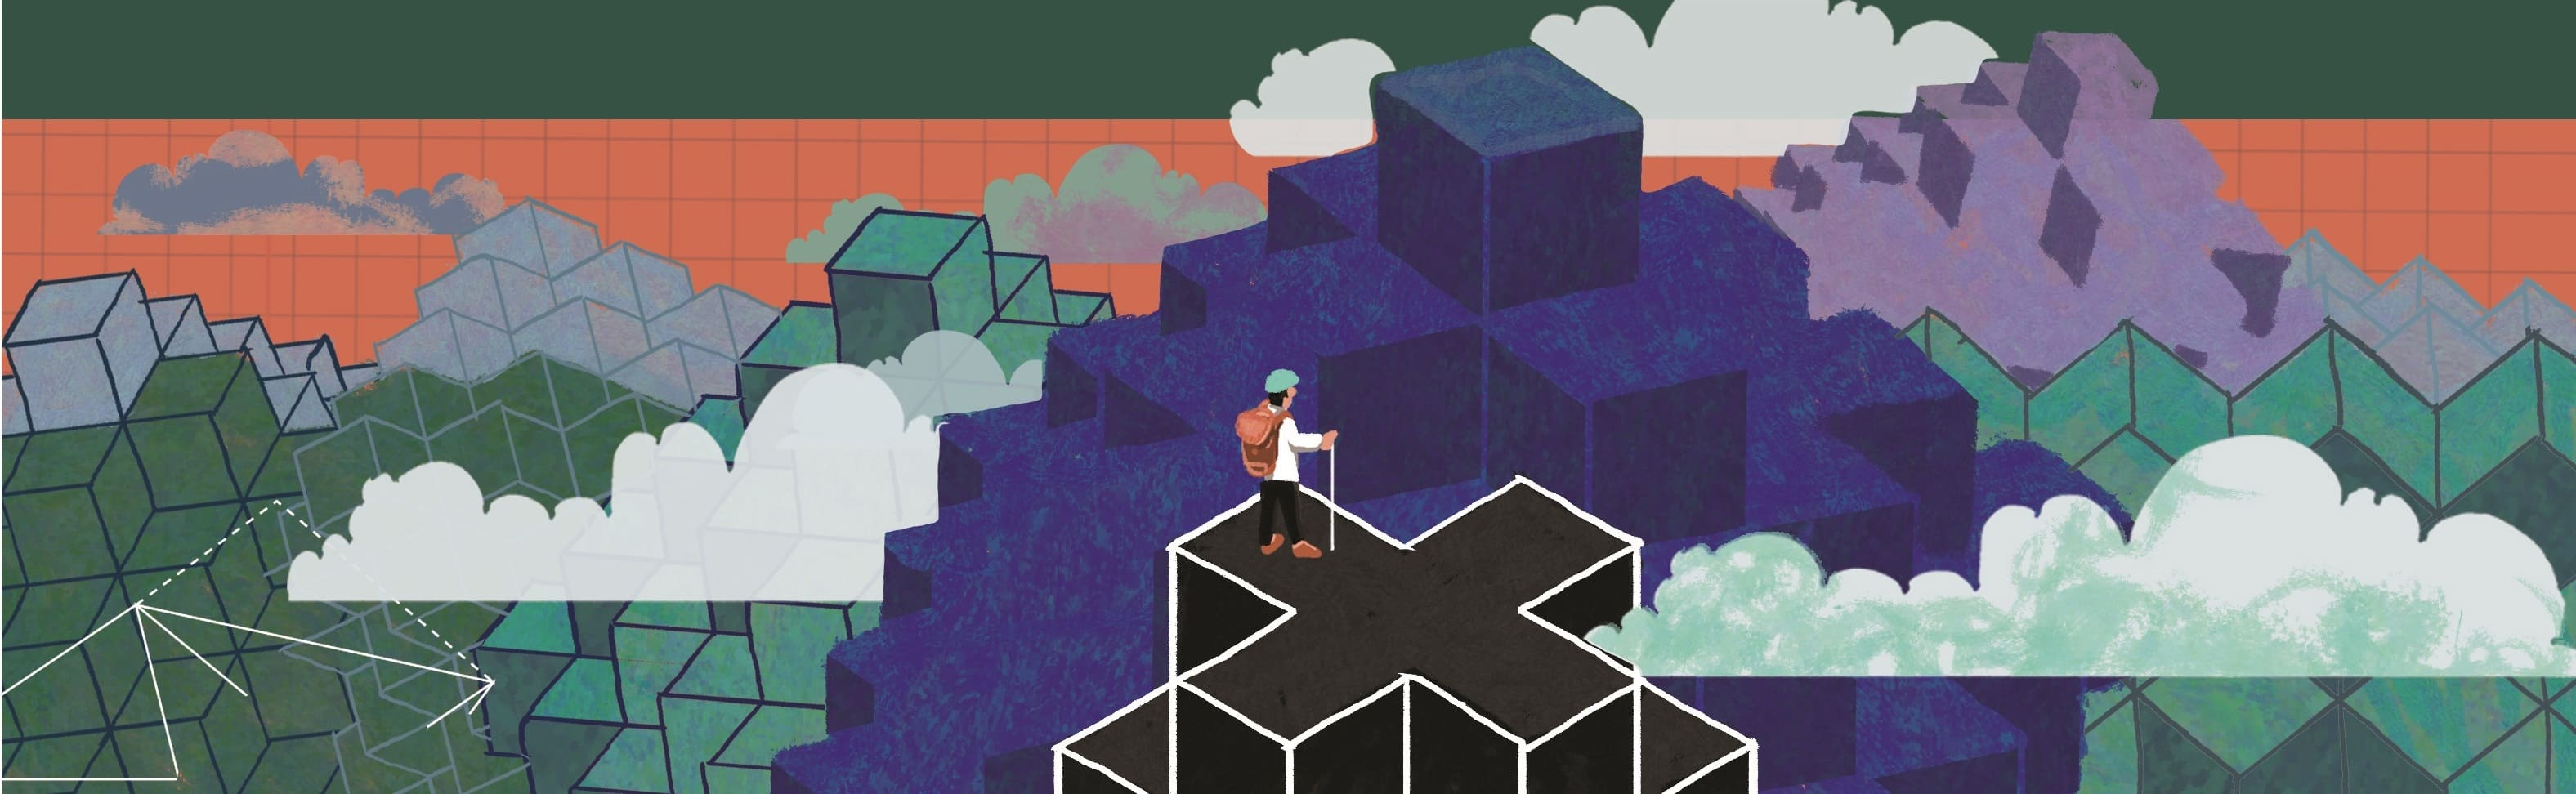
\includegraphics[width=19.3cm]{../thachthuctoanhoc/bannerthachthuc}}}
\centering
\vspace*{4cm}
\endgroup
\vspace*{-8pt}
\begin{tBox}
	\begin{itemize}[leftmargin = 13pt, itemsep = 1.0pt] 
		\item Mỗi bài toán đề xuất (kèm theo lời giải) cần được nêu rõ là bài sáng tác hay bài sưu tầm.
		%		\item Mỗi bài toán đề xuất (kèm theo lời giải) cần được nêu rõ là bài sáng tác hay bài sưu tầm (nếu là bài sưu tầm, cần ghi rõ nguồn).
		\item Bài giải cho mỗi bài toán cần được trình bày trong một file riêng hoặc
		một tờ giấy riêng.
		\item  Người đề xuất bài toán hoặc gửi bài giải cho các bài toán trong mục ``Thách thức kỳ này" cần ghi rõ họ, đệm, tên và nơi làm việc/học tập, số điện thoại liên hệ. Nếu là học sinh (hoặc sinh viên) cần ghi rõ là học sinh lớp mấy (hoặc sinh viên năm thứ mấy).
		\item Các bài toán trong mục Thách thức kỳ này hướng tới các độc giả là học sinh phổ thông; được phân chia thành các mức độ $B$, $A$, và được sắp xếp theo độ khó tăng dần, theo đánh giá chủ quan của Ban biên tập. Các bài toán mức độ $B$ không đòi hỏi các kiến thức vượt quá chương trình môn Toán cấp THCS; các bài toán mức độ $A$ không đòi hỏi các kiến thức vượt quá chương trình môn Toán cấp THPT.
		\item Cách thức gửi bài toán đề xuất hoặc lời giải: gửi file thu được bằng cách scan, ảnh chụp (rõ nét) của bản viết tay, hoặc được soạn thảo bằng các phần mềm Latex, Word tới \url{bbt@pi.edu.vn} hoặc gửi qua đường bưu điện tới Tòa soạn (xem địa chỉ tại bìa $2$).
		\item Hạn gửi lời giải cho các bài toán P$731$--P$740$: trước ngày $15/10/2023$.
	\end{itemize}
\end{tBox}
\begin{center}
	\vspace*{-5pt}
	\textbf{\color{thachthuctoanhoc}\color{thachthuctoanhoc}\color{thachthuctoanhoc}\color{thachthuctoanhoc}THÁCH THỨC KỲ NÀY}
	\vspace*{-5pt}
\end{center}
\begin{multicols}{2}
	\setlength{\abovedisplayskip}{4pt}
	\setlength{\belowdisplayskip}{4pt}
	{\color{thachthuctoanhoc}{\usefont{T5}{qag}{b}{n} P731.}}
	(Mức $B$) Ghép $9$ hình vuông thành một hình chữ nhật như ở hình dưới đây. Biết rằng, hình vuông màu đen có cạnh bằng $1$. Tìm chiều dài và chiều rộng của hình chữ nhật.
	\begin{figure}[H]
		\vspace*{-5pt}
		\centering
		\captionsetup{labelformat= empty, justification=centering}
		\begin{tikzpicture}[thachthuctoanhoc,scale=0.15]
				\draw[fill=black] (0,0) rectangle (1,1);
				\draw  (0.,-9.)-- (9.,-9.);
				\draw  (9.,-9.)-- (9.,0.);
				\draw  (9.,0.)-- (0.,0.);
				\draw  (0.,0.)-- (0.,-9.);
				\draw  (1.,0.)-- (9.,0.);
				\draw  (9.,0.)-- (9.,8.);
				\draw  (9.,8.)-- (1.,8.);
				\draw  (1.,8.)-- (1.,0.);
				\draw  (-10.,-9.)-- (0.,-9.);
				\draw  (0.,-9.)-- (0.,1.);
				\draw  (0.,1.)-- (-10.,1.);
				\draw  (-10.,1.)-- (-10.,-9.);
				\draw  (-6.,1.)-- (1.,1.);
				\draw  (1.,1.)-- (1.,8.);
				\draw  (1.,8.)-- (-6.,8.);
				\draw  (-6.,8.)-- (-6.,1.);
				\draw  (-10.,1.)-- (-6.,1.);
				\draw  (-6.,1.)-- (-6.,5.);
				\draw  (-6.,5.)-- (-10.,5.);
				\draw  (-10.,5.)-- (-10.,1.);
				\draw  (-6.,8.)-- (9.,8.);
				\draw  (9.,8.)-- (9.,23.);
				\draw  (9.,23.)-- (-6.,23.);
				\draw  (-6.,23.)-- (-6.,8.);
				\draw  (-24.,-9.)-- (-10.,-9.);
				\draw  (-10.,-9.)-- (-10.,5.);
				\draw  (-10.,5.)-- (-24.,5.);
				\draw  (-24.,5.)-- (-24.,-9.);
				\draw  (-24.,5.)-- (-6.,5.);
				\draw  (-6.,5.)-- (-6.,23.);
				\draw  (-6.,23.)-- (-24.,23.);
				\draw  (-24.,23.)-- (-24.,5.);	
		\end{tikzpicture}
		\vspace*{-10pt}
	\end{figure} 
	\begin{flushright}
		\textit{Bùi Văn Biên, France (st)}
	\end{flushright}
	{\color{thachthuctoanhoc}{\usefont{T5}{qag}{b}{n} P732.}}
	(Mức $B$) Xét $4$ số thực (không nhất thiết đôi một khác nhau), mà mỗi số có trị tuyệt đối không vượt quá $\dfrac12$, và tổng của ba số bất kỳ, trong bốn số đó, là một số nguyên. Tìm tất cả các giá trị có thể của tổng bốn số đó.
	\begin{flushright}
		\textit{Nguyễn Đức Tấn, Tp. Hồ Chí Minh (st)}
	\end{flushright}
	{\color{thachthuctoanhoc}{\usefont{T5}{qag}{b}{n} P733.}}
	(Mức $B$) Tìm giá trị nhỏ nhất của biểu thức
	\begin{align*}
		S=\left\lfloor\dfrac{b+c}a\right\rfloor+\left\lfloor\dfrac{c+a}b\right\rfloor+\left\lfloor\dfrac{a+b}c\right\rfloor
	\end{align*}
	trong đó $a,b,c$ là các biến nguyên dương,$\lfloor x\rfloor$ ký hiệu số nguyên lớn nhất không vượt quá $x$.
	\begin{flushright}
		\textit{Nguyễn Việt Hùng, Hà Nội (st)}
	\end{flushright}
	
	{\color{thachthuctoanhoc}{\usefont{T5}{qag}{b}{n} P734.}}
	(Mức $B$) Cho hình vuông $ABCD$. Gọi $E$ là trung điểm của $AD$; $H$ là hình chiếu vuông góc của $B$ trên $CE$. Trên đường chéo $AC$, lấy điểm $M$ sao cho $AM=\dfrac38AC$. Chứng minh rằng, $ME$ song song với $DH$.  
	\begin{center}
		\definecolor{ffvvqq}{rgb}{1,0.3333333333333333,0}
		\definecolor{qqzzcc}{rgb}{0,0.6,0.8}
		\definecolor{qqqqff}{rgb}{0,0,1}
		\definecolor{qqqqffa}{rgb}{1,1,1}
		\begin{tikzpicture}[thachthuctoanhoc,scale=0.75]
			\draw [color=qqzzcc] (-3.3,3.3)-- (2.7,3.3);
			\draw [color=qqzzcc] (-3.3,3.3)-- (-3.3,-2.7);
			\draw [color=qqzzcc] (-3.3,-2.7)-- (2.7,-2.7);
			\draw [color=qqzzcc] (2.7,-2.7)-- (2.7,3.3);
			\draw  (-3.3,0.3)-- (2.7,-2.7);
			\draw  (0.3,-1.5)-- (2.7,3.3);
			\draw  (-3.3,-2.7)-- (0.3,-1.5);
			\draw [color=ffvvqq] (-3.3,3.3)-- (2.7,-2.7);
			\draw  (-3.3,0.3)-- (-1.05,1.05);
			\draw [fill=white] (-3.3,3.3) circle (1.6pt);
			\draw (-3.44,3.79) node {$A$};
			\draw [fill=white] (2.7,3.3) circle (1.6pt);
			\draw (2.72,3.71) node {$B$};
			\draw [fill=white] (2.7,-2.7) circle (1.6pt);
			\draw (2.68,-3.05) node {$C$};
			\draw [fill=white] (-3.3,-2.7) circle (1.6pt);
			\draw (-3.36,-3.09) node {$D$};
			\draw [fill=white] (-3.3,0.3) circle (1.6pt);
			\draw (-3.76,0.47) node {$E$};
			\draw [fill=white] (0.3,-1.5) circle (1.6pt);
			\draw (0.3,-1.85) node {$H$};
			\draw [fill=white] (-1.05,1.05) circle (1.6pt);
			\draw (-0.76,1.49) node {$M$};
		\end{tikzpicture}
	\end{center}
	\begin{flushright}
		\textit{Huỳnh Thanh Hưng, Phú Yên}
	\end{flushright}
	{\color{thachthuctoanhoc}{\usefont{T5}{qag}{b}{n} P735.}}
	(Mức $B$) Tìm tất cả các số nguyên dương $n$, để $n!+n$ là một luỹ thừa với số mũ nguyên dương của một số nguyên tố.
	\begin{flushright}
		\textit{Hà Duy Hưng, Hà Nội}
	\end{flushright}
	{\color{thachthuctoanhoc}{\usefont{T5}{qag}{b}{n} P736.}}
	(Mức $B$) Bạn An có $8$ quả cân có tổng trọng lượng là $16$ kg và trọng lượng mỗi quả, theo đơn vị kg, là một số nguyên dương không vượt quá $8$. Chứng minh rằng, có thể chia $8$ quả cân này thành hai nhóm sao cho các tổng trọng lượng của các quả cân cùng nhóm bằng nhau.
	\begin{flushright}
		\textit{Tường Thanh, Nghệ An}
	\end{flushright}
	{\color{thachthuctoanhoc}{\usefont{T5}{qag}{b}{n} P737.}}
	(Mức $A$) Xét các số thực dương $a,b,c$,  thoả mãn $a^2+b^2+c^2=1$. Tìm giá trị nhỏ nhất của biểu thức
	\begin{align*}
		S=2\left(a^3+b^3+c^3\right)-\left(a+b+c\right).
	\end{align*}
	\begin{flushright}
		\textit{Kiều Đình Minh, Phú Thọ}
	\end{flushright}
	{\color{thachthuctoanhoc}{\usefont{T5}{qag}{b}{n} P738.}}
	(Mức $A$) Cho tam giác $ABC$ ngoại tiếp đường tròn $(I)$. Gọi $J$ là tâm đường tròn bàng tiếp góc $A$ của tam giác đó. Trên cạnh $BC$, lấy điểm $D$ tùy ý, sao cho ba điểm $A,I,D$ không thẳng hàng. Đường thẳng $AD$ cắt các đường thẳng $IB, IC$, tương ứng, tại $E,F$. Gọi $H$ là trực tâm của tam giác $IEF$, và gọi $K$ là trung điểm của $AD$. Chứng minh ba điểm $K, H, J$ thẳng hàng.
	\begin{center}
		\definecolor{ffvvqq}{rgb}{1,0.3333333333333333,0}
		\definecolor{qqzzcc}{rgb}{0,0.6,0.8}
		\definecolor{qqqqff}{rgb}{0,0,1}
		\definecolor{qqqqffa}{rgb}{1,1,1}
		\definecolor{cqcqcq}{rgb}{0.7529411764705882,0.7529411764705882,0.7529411764705882}
		\begin{tikzpicture}[thachthuctoanhoc,scale=0.45]
			\draw [color=qqzzcc] (-3.679901022761026,4.943589529660562)-- (-4.58,-1.6);
			\draw [color=qqzzcc] (-4.58,-1.6)-- (3.08,-1.6);
			\draw [color=qqzzcc] (3.08,-1.6)-- (-3.679901022761026,4.943589529660562);
			\draw [color=ffvvqq] (-3.257494355051633,-1.6)-- (-3.679901022761026,4.943589529660562);
			\draw [color=ffvvqq] (-4.58,-1.6)-- (-2.151513063456181,0.5173053476685014);
			\draw [color=ffvvqq] (-3.4275087350979017,1.0337281160719551)-- (3.08,-1.6);
			\draw [dashed] (-3.4686976889063295,1.671794764830281)-- (0.6515130634561829,-7.600391557576506);
			\draw  (-2.151513063456181,0.5173053476685014) circle (2.117305347668501cm);
			\draw  (0.6515130634561829,-7.600391557576506) circle (6.000391557576506cm);
			\draw [color=qqzzcc] (-4.58,-1.6)-- (-5.292904303746716,-6.782711296880436);
			\draw [color=qqzzcc] (3.08,-1.6)-- (4.824890183355734,-3.2890550757724784);
			\draw [fill=white] (-3.679901022761026,4.943589529660562) circle (2.5pt);
			\draw (-3.7075216945790075,5.430778676473025) node {$A$};
			\draw [fill=white] (-4.58,-1.6) circle (2.5pt);
			\draw (-5.171417300932007,-1.6163200271099578) node {$B$};
			\draw [fill=white] (3.08,-1.6) circle (2.5pt);
			\draw (3.5014736499140704,-1.2848719652941842) node {$C$};
			\draw [fill=white] (-2.151513063456181,0.5173053476685014) circle (2.5pt);
			\draw (-1.9397986982282145,0.012402451962288) node {$I$};
			\draw [fill=white] (0.6515130634561829,-7.600391557576506) circle (2.5pt);
			\draw (0.6565444526620129,-8.41453873427639) node {$J$};
			\draw [fill=white] (-3.257494355051633,-1.6) circle (2.5pt);
			\draw (-3.3484529609452527,-2.058250776197656) node {$D$};
			\draw [fill=white] (-3.4686976889063295,1.671794764830281) circle (2.5pt);
			\draw (-2.80379702736733282,1.9124706683174956) node {$K$};
			\draw [fill=white] (-3.327960493319134,-0.5083943985466047) circle (2.5pt);
			\draw (-2.84462557094746,-0.667344980266746) node {$E$};
			\draw [fill=white] (-3.4275087350979017,1.0337281160719551) circle (2.5pt);
			\draw (-3.818004381850932,0.9800231237802691) node {$F$};
			\draw [fill=white] (-2.9332617149580074,0.4668413261447786) circle (2.5pt);
			\draw (-2.685556837313705,0.8842990928723823) node {$H$};
			\draw [fill=white] (0.6515130634561829,-1.6) circle (2.5pt);
			\draw [fill=white] (-5.292904303746716,-6.782711296880436) circle (2.5pt);
			\draw [fill=white] (4.824890183355734,-3.2890550757724784) circle (2.5pt);
		\end{tikzpicture}
	\end{center}
	\begin{flushright}
		\textit{Lưu Công Đông, Hà Nội}
	\end{flushright}
	{\color{thachthuctoanhoc}{\usefont{T5}{qag}{b}{n} P739.}}
	(Mức $A$) Cho dãy số $(a_n)$, xác định bởi
	\begin{align*}
		a_n=\left\lfloor\dfrac n{\sqrt2}\right\rfloor+\left\lfloor\dfrac n{\sqrt3}\right\rfloor,\quad\text{với mọi $n\in\mathbb N^*$}.
	\end{align*}
	Trong đó, $\lfloor x\rfloor$ ký hiệu số nguyên lớn nhất không vượt quá $x$.
	Chứng minh rằng, trong dãy $(a_n)$ có vô hạn số chẵn và vô hạn số lẻ.
	\begin{flushright}
		\textit{Nguyễn Tiến Lâm, Hà Nội}
	\end{flushright}
	{\color{thachthuctoanhoc}{\usefont{T5}{qag}{b}{n} P740.}}
	(Mức $A$) Cho bảng ô vuông kích thước $2023\times 2023$. Tìm số nguyên dương $n$ nhỏ nhất, sao cho có thể đặt $n$ viên bi vào các ô vuông con của bảng, đảm bảo các điều kiện sau được đồng thời thoả mãn:
	\vskip 0.1cm
	$i/$ Ở mỗi ô vuông con chỉ có tối đa một viên bi;
	\vskip 0.1cm
	$ii/$ Với mỗi ô vuông con không có bi, tổng số viên bi ở hàng và cột chứa ô đó không nhỏ hơn $2023$.
	\begin{flushright}
		\textit{Tô Trung Hiếu, Nghệ An (st)}
	\end{flushright}
\end{multicols}
\newpage
\centerline{{\large{\textbf{\color{thachthuctoanhoc}\color{thachthuctoanhoc}GIẢI BÀI KỲ TRƯỚC}}}}
\vspace*{-5pt}
\begin{multicols}{2}
	{\color{thachthuctoanhoc}{\usefont{T5}{qag}{b}{n} P678.}}
	Trong mặt phẳng, cho hai điểm $I$, $J$ cố định thoả mãn $IJ=8$.  Gọi $(S)$ là tập hợp các điểm $M$ sao cho ít nhất một trong hai đoạn thẳng $MI,MJ$ có độ dài không vượt quá $7$. Với $A,B,C$ là ba điểm không thẳng hàng thuộc $(S)$, chu vi tam giác $ABC$ lớn nhất là bao nhiêu?
	\vskip 0.05cm
	Bài toán {\color{thachthuctoanhoc}{\usefont{T5}{qag}{b}{n} P678}}, được thầy Trần Quốc Luật, trường THPT chuyên Lê Hồng Phong, Tp Hồ Chí Minh, đề xuất trong số báo $1-2$ năm $2023$. Đây là một bài toán khó và thực tế là Tạp chí chỉ nhận được duy nhất một lời giải từ phía bạn đọc. Trong số này, chúng tôi giới thiệu với bạn đọc hai lời giải với hai hướng tiếp cận khác nhau. 
	\vskip 0.05cm
	\textbf{\color{thachthuctoanhoc}Lời giải $\pmb{1.}$} Trước tiên ta có các nhận xét sau:
	\vskip 0.05cm
	\textit{Nhận xét $1$.} Tập hợp $(S)$ là tập hợp các điểm nằm trong hoặc nằm trên một trong hai đường tròn $(I;7)$ hoặc $(J;7)$. 
	\vskip 0.05cm
	Gọi $M,N$ là giao điểm của hai đường tròn này. Khi đó, biên $\partial S$ của $S$ là hợp của $\partial S_1$ và $\partial S_2$, trong đó $\partial S_1$ là cung lớn $MN$ của $(I)$ và $\partial S_2$ là cung lớn $MN$ của $(J)$.
 	\vskip 0.05cm	
	Ký hiệu $P_{XYZ}$ là chu vi tam giác $XYZ$.
	\vskip 0.05cm
	\textit{Nhận xét $2$.} Đối với tam giác $ABC$ bất kỳ, nếu $A'$ nằm trên tia $BA$ và nằm ngoài đoạn $BA$ thì $P_{A'BC}> P_{ABC}$. 
	\vskip 0.05cm
	Trước tiên ta rút gọn về trường hợp tam giác có ba đỉnh nằm trên biên của $S$.
	\vskip 0.05cm
	Xét tam giác $ABC$ với $A,B,C$ là ba điểm thuộc $(S)$. Giả sử tam giác $ABC$ có một đỉnh nằm hoàn toàn bên trong $S$. Chẳng hạn $A\in S\setminus \partial S$. Tia $BA$ cắt $\partial S$ tại không quá $4$ điểm (thực ra là $3$); gọi $A'$ là giao điểm có khoảng cách tới $B$ là lớn nhất (nếu có nhiều hơn $1$ giao điểm). Ta có $A'$ nằm ngoài đoạn thẳng $BA$, vì thế theo nhận xét $2$ thì $P_{A'BC}> P_{ABC}$. Tiếp tục lập luận như vậy với $B$ nếu $B\notin \partial S$ (cho tam giác $A'BC$), rồi với $C$ nếu $C\notin \partial S$. Các suy luận trên cho thấy nếu một trong $3$ đỉnh $A, B, C$ không nằm trên biên của $S$ thì ta có thể tìm được một tam giác mới (có các đỉnh thuộc $\partial S$) có chu vi lớn hơn chu vi tam giác $ABC$.
	\vskip 0.05cm
	Bây giờ, xét trường hợp tam giác $ABC$ có các đỉnh thuộc $\partial S$. Do $\partial S = \partial S_1 \cup \partial S_2$ nên có $2$ trường hợp xảy ra: Trường hợp $1)$ có $2$ đỉnh nằm trên một cung và đỉnh thứ $3$ nằm trên cung còn lại; Trường hợp $2)$ cả $3$ đỉnh cùng nằm trên cùng một cung (nói riêng cùng nằm trên một đường tròn).
	\vskip 0.05cm
	\textit{Trường hợp $1.$} Không giảm tổng quát, giả sử $A$ thuộc $\partial S_1$ và $B,C$ thuộc $\partial S_2$. 
	\vskip 0.05cm	
	Đặt $2\alpha=(\vec{JC}, \vec{JB})$, $2\beta=(\vec{JA}, \vec{JC})$, $2\gamma= (\vec{JB}, \vec{JA})$. Như vậy, $2\alpha + 2 \beta + 2\gamma \equiv 0\pmod{2\pi}$, hay $\alpha + \beta + \gamma \equiv 0 \pmod{\pi}$.
	\vskip 0.05cm
	Đặt $t=AJ$. Như vậy, $t>0$ và 
	\begin{align*}
		t\leq AI+JI=15.
	\end{align*}
	\begin{center}
		\definecolor{qqqqff}{rgb}{0,0,1}
		\definecolor{qqqqffa}{rgb}{1,1,1}
		\begin{tikzpicture}[thachthuctoanhoc,scale=0.55]
			\draw [shift={(3,0.4)}] (0,0) -- (-76.37300514010846:0.4) arc (-76.37300514010846:65.35609953429524:0.4) -- cycle;
			\draw  (-2,0.4) circle (4cm);
			\draw  (3,0.4) circle (4cm);
			\draw  (0.5,3.522498999199199)-- (0.5,-2.7224989991991992);
			\draw  (-4.611364135838608,3.4299797606676976)-- (4.667909334714851,4.035667538591924);
			\draw  (4.667909334714851,4.035667538591924)-- (3.9424001024860162,-3.487400422754819);
			\draw  (3.9424001024860162,-3.487400422754819)-- (-4.611364135838608,3.4299797606676976);
			\draw  (-4.611364135838608,3.4299797606676976)-- (3,0.4);
			\draw  (3,0.4)-- (4.667909334714851,4.035667538591924);
			\draw  (3,0.4)-- (3.9424001024860162,-3.487400422754819);
			\draw (3.38,0.92) node[anchor=north west] {$2\alpha$};
			\draw [fill=white] (-2,0.4) circle (2.6pt);
			\draw (-1.98,-0.2) node {$I$};
			\draw [fill=white] (3,0.4) circle (2.6pt);
			\draw (2.72,-0.2) node {$J$};
			\draw [fill=white] (0.5,3.522498999199199) circle (2.6pt);
			\draw (0.46,4.2) node {$M$};
			\draw [fill=white] (0.5,-2.7224989991991992) circle (2.6pt);
			\draw (0.5,-3.2) node {$N$};
			\draw [fill=white] (-4.611364135838608,3.4299797606676976) circle (2.6pt);
			\draw (-4.94,3.75) node {$A$};
			\draw [fill=white] (3.9424001024860162,-3.487400422754819) circle (2.6pt);
			\draw (3.88,-4) node {$C$};
			\draw [fill=white] (4.667909334714851,4.035667538591924) circle (2.6pt);
			\draw (4.68,4.57) node {$B$};
		\end{tikzpicture}
	\end{center}
	Theo định lý cosin (hoặc đơn giản sử dụng véc tơ: $AB^2  = (\vec{JA}- \vec{JB})^2$), ta có 
	\begin{align*}
		&AB^2=t^2+7^2-14t\cos 2\gamma,\\
		&AC^2=t^2+7^2-14t \cos2\beta.
	\end{align*}
	Suy ra 
	\begin{align*}
		&AB^2+AC^2\\
		= \,&2t^2+98-14t \left( \cos2\gamma +\cos 2\beta \right)\\
		= \,&2t^2+98-28t\cos (\beta+ \gamma)\cos (\beta-\gamma)\\
		= \,&2t^2+98\pm 28t\cos\alpha \cos (\beta-\gamma)\\
		\leq \,&2\cdot 15^2 + 98 + 28\cdot 15 |\cos \alpha| \\
		= \,&548+420 |\cos\alpha|.
	\end{align*}
	Từ đó, theo bất đẳng thức Cauchy--Schwarz 
	\begin{align*}
		AB+AC &\leq \sqrt{2(AB^2+AC^2)}\\
		&=2\sqrt{274+210|\cos\alpha|} . 
	\end{align*}
	Lại có, vẫn theo định lý cosin, 
	\begin{align*}
		BC^2 &=7^2+7^2-2\cdot 7\cdot 7 \cos2\alpha\\
		&= 2\cdot 7^2 - 2\cdot 7^2 (1-2\sin^2 \alpha)\\
		& = 4\cdot 7^2\cdot \sin^2\alpha.
	\end{align*}
	Do đó $BC=14 | \sin\alpha|$. Vậy,
	\begin{align*}
			P_{ABC}\leq 14| \sin\alpha|+2\sqrt{274+210|\cos\alpha|}.
	\end{align*}
	Đặt $r=|\cos\alpha|$ thì $P_{ABC}\le g(r)$, trong đó
	\begin{align*}
		g(r)=14\sqrt{1-r^2}+2\sqrt{274+210r}.
	\end{align*}
	Ta sẽ tìm giá trị lớn nhất của hàm số $g(r)$ trên $[0;1]$. Đây là một hàm số liên tục, có đạo hàm trên $(0, 1)$. Ta biết rằng $g$ đạt cực đại trên $[0; 1]$; hơn nữa, nếu $g$ đạt cực đại tại một điểm $r_0$ thì hoặc $r_0$ là một giá trị biên (nghĩa là $r_0=0$ hoặc $r_0=1$) hoặc $r_0$ là một điểm bên trong mà tại đó đạo hàm triệt tiêu ($r_0\in (0, 1)$ và là một nghiệm của đạo hàm).
	Ta có
	\begin{align*}
		g^\prime(r)=-\dfrac{14r}{\sqrt{1-r^2}}+\dfrac{210}{\sqrt{274+210r}}.
	\end{align*}
	Từ đó, $g'(r)=0$ khi và chỉ khi $14 r \sqrt{274 + 210r}= 210 \sqrt{1-r^2}$, hay một cách tương đương $ r \sqrt{274+ 210r}= 15 \sqrt{1-r^2}$. Bình phương hai vế và chuyển vế, ta thu được $210 r^3 + 499 r^2 - 225=0$, hay
	\begin{align*}
		(5r-3)(6r+5)(7r+15)=0.
	\end{align*} 
	Điều này có nghĩa là $r_0=\dfrac{3}{5}$ là điểm duy nhất trong khoảng $(0,1)$ mà ở đó đạo hàm của $g$ triệt tiêu. Cuối cùng, nhận xét rằng $g(0)= 14 + 2\sqrt{274}, g\left(\dfrac{3}{5}\right) = \dfrac{256}{5}, g(1)= 44$ nên giá trị lớn nhất của $g$ trên $[0; 1]$ bằng $\dfrac{256}{5}$, đạt được tại $r= \dfrac{3}{5}$. 
	\vskip 0.05cm
	Từ đó suy ra $P_{ABC}\le \dfrac{256}{5}$. Dấu ``$=$" đạt được khi $ABC$ là tam giác cân, với $A$ là giao điểm của $IJ$ và $(I)$ sao cho $I$ nằm giữa $A$ và $J$; và $B, C$ là các giao điểm với $(J)$ của đường tròn tâm $A$, bán kính $ \sqrt{274 + 210 \cdot \dfrac{3}{5}}=20$.
	\vskip 0.05cm
	\textit{Trường hợp $2.$} Cả ba điểm $A, B, C$ cùng nằm trên một đường tròn, chẳng hạn là đường tròn $(I;7)$. Lúc này, 
	\begin{align*}
		P_{ABC}&=2\cdot 7 \cdot (\sin A+\sin B+\sin C)\le 6\cdot 7\\ &=42<\dfrac{256}{5}.
	\end{align*}
	Từ các lập luận trên, ta suy ra tam giác $ABC$ có chu vi lớn nhất là $\dfrac{256}{5}$. 
	\vskip 0.05cm
	\textbf{\color{thachthuctoanhoc}Lời giải} $\pmb{2}$ (\textit{của bạn Trần Minh Hoàng, học sinh lớp $10$, trường THPT chuyên Hà Tĩnh})\textbf{\color{thachthuctoanhoc}.}
	\vskip 0.1cm
	Ta sử dụng hai bổ đề sau:
	\vskip 0.1cm
	\textbf{\color{thachthuctoanhoc}Bổ đề $\pmb{1.}$} Cho elíp $(E)$ có hai tiêu điểm $F_1,F_2$. Lấy điểm $M$ bất kỳ nằm trên $(E)$ và điểm $N$ bất kỳ nằm ngoài elíp này. Khi đó $MF_1+MF_2 < NF_1+NF_2$.
	\begin{figure}[H]
		\vspace*{-5pt}
		\centering
		\captionsetup{labelformat= empty, justification=centering}
		\definecolor{xdxdff}{rgb}{0.49019607843137253,0.49019607843137253,1.}
		\definecolor{ududff}{rgb}{0.30196078431372547,0.30196078431372547,1.}
		\begin{tikzpicture}[thachthuctoanhoc,scale=0.85]
			\draw [rotate around={0.:(0.5,2.)}] (0.5,2.) ellipse (2.4555339953435182cm and 1.9441314776238001cm);
			\draw  (1.4265834936058992,3.8004071913071167)-- (2.,2.);
			\draw  (-1.,2.)-- (3.0154057379903705,4.979236191848852);
			\draw [fill=white] (-1.,2.) circle (1.5pt);
			\draw (-1.05,1.64) node {$F_1$};
			\draw [fill=white] (2.,2.) circle (1.5pt);
			\draw (2.11,1.58) node {$F_2$};
			\draw [fill=white] (0.34,3.94) circle (1.5pt);
			\draw (0.42,4.33) node {$M$};
			\draw [fill=white] (1.4265834936058992,3.8004071913071167) circle (1.5pt);
			\draw (1.38,4.31) node {$U$};
			\draw [fill=white] (3.0154057379903705,4.979236191848852) circle (1.5pt);
			\draw (3.12,4.67) node {$N$};
		\end{tikzpicture}
		\vspace*{-10pt}
	\end{figure}
	\textit{Chứng minh.} Đoạn thẳng $NF_1$, có một đầu mút nằm bên trong và một đầu mút nằm bên ngoài elíp, do đó cắt $(E)$ tại một điểm nào đó, ký hiệu là $U$.
	Rõ ràng $N$ không thể thuộc đoạn thẳng $UF_2$. Do đó, ta có $MF_1+MF_2 = UF_1+UF_2 < UF_1 + UN+NF_2 = NF_1 + NF_2$. 
	\vskip 0.05cm
	\textbf{\color{thachthuctoanhoc}Bổ đề $\pmb{2.}$} Cho elíp $(E)$ có hai tiêu điểm $F_1,F_2$ và điểm $M$ bất kỳ thuộc $(E)$. Khi đó phân giác ngoài của $\angle{F_1MF_2}$ tiếp xúc với $(E)$.
	\begin{figure}[H]
		\vspace*{-10pt}
		\centering
		\captionsetup{labelformat= empty, justification=centering}
		\definecolor{xdxdff}{rgb}{0.49019607843137253,0.49019607843137253,1.}
		\definecolor{uuuuuu}{rgb}{0.26666666666666666,0.26666666666666666,0.26666666666666666}
		\definecolor{ududff}{rgb}{0.30196078431372547,0.30196078431372547,1.}
		\begin{tikzpicture}[thachthuctoanhoc,scale=0.85]
			\draw [rotate around={0.:(0.5,2.)}] (0.5,2.) ellipse (2.4555339953435182cm and 1.9441314776238001cm);
			\draw  (-1.,2.)-- (0.34,3.94);
			\draw  (-1.1929115093255551,5.73147489644071)-- (-1.,2.);
			\draw  (-1.1929115093255551,5.73147489644071)-- (2.,2.);
			\draw  (0.34,3.94)-- (2.087515517856266,4.030343862809057);
			\draw [fill=white] (-1.,2.) circle (1.5pt);
			\draw (-1.040678263775316,1.61691538002340639) node {$F_1$};
			\draw [fill=white] (2.,2.) circle (1.5pt);
			\draw (2.1012386841826762,1.6140324502698885) node {$F_2$};
			\draw [fill=white] (0.34,3.94) circle (1.5pt);
			\draw (0.42003751027532965,4.29554900692543) node {$M$};
			\draw [fill=white] (-1.1929115093255551,5.73147489644071) circle (2.0pt);
			\draw[color=uuuuuu] (-1.1325471803822749,6.252356930653653) node {$F_3$};
			\draw [fill=white] (2.087515517856266,4.030343862809057) circle (1.5pt);
			\draw (2.2206682757717227,4.369044140210997) node {$N$};
		\end{tikzpicture}
		\vspace*{-10pt}
	\end{figure}
	\textit{Chứng minh.} Giả sử phân giác ngoài của $\angle{F_1MF_2}$ cắt $(E)$ tại điểm $N$ khác $M$. Lấy $F_3$ đối xứng với $F_1$ qua $MN$. Thế thì $F_3,M,F_2$ thẳng hàng. Do $N\not\equiv M$ nên $N\not\in F_2F_3$, theo bất đẳng thức tam giác ta có: 
	\begin{align*}
		NF_1+NF_2&=NF_3+NF_2 >F_3F_2\\&=MF_3+MF_2=MF_1+MF_2.
	\end{align*}
	Điều này là vô lý do $M,N$ đều thuộc $(E)$. Do đó giả sử trên là sai, hay ta có phân giác ngoài của $\angle{F_1MF_2}$ tiếp xúc với $(E)$.
	\vskip 0.1cm
	\textit{Quay trở lại bài toán:}
	\begin{center}
	\begin{tikzpicture}[scale=0.28, thachthuctoanhoc]
		\draw(-4.,0.) circle (7cm);
		\draw (-4.,0.)-- (4.,0.);
		\draw(4.,0.) circle (7cm);
		\draw (-11.,0.)-- (8.2,5.6);
		\draw (-11.,0.)-- (8.2,-5.6);
		\draw (8.2,5.6)-- (8.2,-5.6);
		\draw (-11.,0.)-- (-4.,0.);
		\draw (4.,0.)-- (8.2,0.);
		\draw (4.,0.)-- (8.2,5.6);
		\draw (4.,0.)-- (8.2,-5.6);
			\draw [fill=white] (-4.,0.) circle (4.5pt);
			\draw (-3.6901287699666807,0.96020769758771811) node {$J$};
			\draw [fill=white] (4.,0.) circle (4.5pt);
			\draw (3.783060241936751,0.644061183809223) node {$I$};
			\draw [fill=white] (-11.,0.) circle (4.5pt);
			\draw (-11.667128277054614,0.5181085600130975) node {$C$};
			\draw [fill=white] (8.2,0.) circle (4.5pt);
			\draw (9.485291530325428,0.6020769758771811) node {$H$};
			\draw [fill=white] (8.2,-5.6) circle (4.5pt);
			\draw (8.611244154121554,-6.47459461521341) node {$A$};
			\draw [fill=white] (8.2,5.6) circle (4.5pt);
			\draw (8.485291530325428,6.85976630838742) node {$B$};
	\end{tikzpicture}
\end{center}
Dễ thấy $(S)$ là hợp của hai hình tròn $(I; 7)$ và $(J; 7)$ (bao gồm cả phần bên trong lẫn biên, là đường tròn tương ứng; để cho tiện ta sẽ ký hiệu $(I)$ cho cả hình tròn và đường tròn tâm $I$ bán kính $7$). Vì chu vi tam giác $ABC$ luôn không vượt quá $3$ lần khoảng cách lớn nhất giữa hai điểm thuộc $(S)$, đồng thời các điểm thuộc $(S)$ có tính liên tục nên ta lấy được ba điểm $A,B,C$ thuộc $(S)$ sao cho chu vi tam giác $ABC$ là lớn nhất. (Cụ thể hơn, nếu gọi $P(X, Y, Z)$ là chu vi của tam giác $XYZ$ thì hàm số $(S) \times (S) \times (S) \to \mathbb{R}$, $(X, Y, Z)\mapsto P(X, Y, Z)$ là một hàm số liên tục và $(S)$ là một tập con đóng và bị chặn nên phải có giá trị lớn nhất).
\vskip 0.1cm
Ta sẽ sử dụng các bổ đề trên để xác định vị trí của $A, B, C$. Gọi $(E_a)$ là elip đi qua $A$ và nhận $B,C$ làm hai tiêu điểm. Các elip $(E_b),(E_c)$ được định nghĩa tương tự.
\vskip 0.1cm
Ta chứng minh rằng mỗi elíp trong $(E_a),(E_b),(E_c)$ tiếp xúc với một trong hai đường tròn $(I),(J)$. 
\vskip 0.1cm
Xét điểm $A$. Do $A\in (S)$, nó thuộc một trong hai hình tròn $(I)$ hoặc $(J)$; không giảm tổng quát, giả sử là $(I)$. Ta sẽ chỉ ra rằng $(E_a)$ tiếp xúc với $(I)$. Thật vậy, giả sử ngược lại $(E_a)$ không tiếp xúc với $(I)$; có nghĩa là $A$ nằm hoàn toàn bên trong đường tròn $(I)$ hoặc  $A$ nằm trên đường tròn $(I)$ nhưng các tiếp tuyến với $(E_a)$ và $(I)$ tại $A$ không trùng nhau. 
\vskip 0.1cm
Kẻ tiếp tuyến $d$ của $(E_a)$ tại $A$. Như vậy, theo giả thiết thì hoặc $A$ nằm hoàn toàn bên trong đường tròn $(I)$, hoặc $A$ nằm trên $(I)$ nhưng $d$ không phải là tiếp tuyến tại $A$ của $(I)$; trong mọi trường hợp $d$ cắt $(I)$ tại ít nhất một điểm $A'$ nào đó không trùng với $A$. Hơn nữa, mọi điểm của tiếp tuyến mà không phải là tiếp điểm thì phải nằm ngoài elíp nên $A'$ nằm ngoài $(E_a)$. Vì thế theo bổ đề $1$, $A'B + A'C > AB+AC$, suy ra chu vi tam giác $ABC$ nhỏ hơn chu vi tam giác $A'BC$, vô lý. 
\vskip 0.1cm
Lập luận trên đây chứng tỏ rằng nếu một đỉnh của tam giác $ABC$ thuộc một trong hai hình tròn thì elíp và đường tròn tương ứng phải tiếp xúc với nhau tại điểm đó. Điều này cho thấy, nói riêng, mỗi đỉnh của tam giác $ABC$ phải nằm trên biên của $(S)$, nghĩa là các phần của các đường tròn $(I), (J)$ không nằm bên miền trong của $(S)$.
\vskip 0.1cm
Theo nguyên lý Dirichlet, hai trong ba đỉnh của tam giác $ABC$ nằm trên biên của $(S)$ thuộc một trong hai đường tròn. Giả sử $A$ và $B$ thuộc đường tròn $(I)$ (và không nằm bên trong $(J)$). Khi đó, như đã thấy, $(I)$ tiếp xúc với $(E_a),(E_b)$ tương ứng tại $A$ và $B$.
\vskip 0.1cm
Theo bổ đề $2$ ta suy ra $AI,BI$ lần lượt là phân giác của $\angle{BAC},\angle{CBA}$. Suy ra $I$ là tâm đường tròn nội tiếp của tam giác $ABC$. Suy ra $CI$ là phân giác $\angle{ACB}$. Mà $\angle IAB= \angle IBA$, nên $\angle BAC = \angle ABC$, hay tam giác $ABC$ cân tại $C$.
\vskip 0.1cm
Xét $2$ trường hợp.
\vskip 0.1cm
\textit{Trường hợp $1$}: $C$ nằm trên đường tròn $(J)$. Khi này, $(E_c)$ tiếp xúc với $(J)$ và tương tự như trên, ta suy ra $CJ$ là phân giác $\angle{ACB}$, nghĩa là $C$ nằm trên đường thẳng $IJ$. Để ý rằng đường thẳng $IJ$ cắt đường tròn $(J)$ tại hai điểm, một điểm nằm trên biên của $(S)$, điểm còn lại nằm hoàn toàn bên trong $(S)$. Theo các lập luận ở phần đầu của lời giải, $C$ phải là điểm nằm trên biên của $(S)$, hay $C$ nằm trên tia đối của tia $JI$. Các dữ kiện trên đây xác định một cách duy nhất tam giác $ABC$ và cho phép chúng ta tính tường minh chu vi của nó như sau.
\vskip 0.1cm
Gọi $H$ là giao điểm của $CI$ và $AB$ và đặt  $x = IH, x > 0$. Ta có $CI = CJ + IJ = 15$ nên $CH = 15 + x$. Suy ra 
\vskip 0.1cm
$ AH^2 = AI^2 - IH^2 = 49 - x^2$, kéo theo $AC^2 = AH^2 + CH^2 = 49 - x^2 + (15 + x)^2 = 274 + 30x$.
\vskip 0.1cm
Mặt khác. vì $AI$ là phân giác $\angle{BAC}$ nên $\dfrac{AH}{AC} = \dfrac{IH}{IC}$, dẫn đến
\vskip 0.1cm
$ \dfrac{AH^2}{AC^2}=\dfrac{IH^2}{IC^2}$, hay $\dfrac{49 - x^2}{274 + 30x} = \dfrac{x^2}{225}$. Từ đó, ta thu được phương trình $ 30x^3 + 499x^2 - 11025=0$, hay $(6 x + 35) (5 x - 21) (x + 15)=0$, dẫn đến $x = \dfrac{21}{5}$.
\vskip 0.05cm
Từ đây, ta tính được $\begin{cases} \!\!\!AC^2 \!=\! 274 \!+\! 30x \!=\! 400 \\ \!\! AH^2 \!=\! 49 \!-\! x^2 \!=\! \dfrac{784}{25}    \end{cases}$ và do đó $\begin{cases} AC = 20 \\ AB = 2AH = \dfrac{56}{5}\end{cases}$.
\vskip 0.05cm
Như vậy, trong trường hợp này, chu vi tam giác $ABC$ bằng $ 2\cdot 20 +    \dfrac{56}{5} = \dfrac{256}{5}$.
\vskip 0.05cm
\textit{Trường hợp $2$}: $C$ nằm trên đường tròn $(I)$. Khi này, tam giác $ABC$ nhận $I$ vừa là tâm đường tròn nội tiếp và tâm đường tròn ngoại tiếp. Dễ thấy $ABC$ phải là tam giác đều và do đó có chu vi bằng
\begin{align*}
	BC+CA+AB = 3\sqrt{3}IA = 21\sqrt{3}	 < \dfrac{256}{5}.
\end{align*}
So sánh hai trường hợp, ta suy ra chu vi tam giác $ABC$ lớn nhất bằng $\dfrac{256}{5}$ và đạt được trong trường hợp $1$.
\vskip 0.05cm
\textbf{\color{thachthuctoanhoc}Bình luận.}
\vskip 0.1cm
Ở lời giải đầu tiên, chúng ta cũng có thể tránh việc sử dụng lượng giác như sau. Như đã thấy, ta quy về trường hợp tam giác $ABC$ có cả ba đỉnh nằm trên biên của $(S)$. Giả sử $B, C$ nằm trên $(I)$ và $A$ nằm trên $(J)$. Gọi $M$ là trung điểm của $BC$ và đặt $x=IM$. Khi này, theo tính chất của đường trung tuyến, ta có
\begin{align*}
	&2(AB^2+AC^2)&\\
	= \,&4AM^2+BC^2= 4(AM^2 + BM^2)\\
	\le\, &4 \left( (IM + JI + AJ)^2 + BM^2\right)\\
	=\,& 4 \left( (x+15)^2 + 7^2-x^2\right)\\
	= \,&4 \left(30x+ 274\right).
\end{align*}
Lưu ý rằng, nếu $A$ nằm trên $(I)$ thay vì $(J)$ thì rõ ràng $AM\le 14< x+15$ nên bất đẳng thức trên cũng đúng. Từ đó suy ra, trong mọi trường hợp thì 
\begin{align*}
	&BC+CA + AB\le BC + \sqrt{2(AB^2+AC^2)}\\
	=\,&2\left(\sqrt{49-x^2} + \sqrt{30x+274}\right).
\end{align*}
Tương tự như lời giải đầu tiên, ta khảo sát hàm số để tìm giá trị lớn nhất của $f(x)$, biểu thức cuối cùng nhận được trên miền xác định của nó là $[0, 7]$. Ta cũng tìm được $x= \dfrac{21}{5}$ là điểm duy nhất trên khoảng $[0, 7]$ mà ở đó đạo hàm triệt tiêu. Sau đó, bằng cách so sánh với các giá trị biên, ta thu được giá trị lớn nhất là $f(\dfrac{21}{5})= \dfrac{256}{5}$. 
	\begin{flushright}
		\textbf{\color{thachthuctoanhoc}Nhóm TTTH}
	\end{flushright}
	{\color{thachthuctoanhoc}{\usefont{T5}{qag}{b}{n} P701.}}
	(Mức $B$) Một chiếc hộp đựng một số viên bi, gồm bi xanh và bi đỏ. Biết rằng, số bi đỏ ít hơn số bi xanh; tổng của số bi xanh và hai lần số bi đỏ lớn hơn $24$; tổng của số bi đỏ và hai lần số bi xanh nhỏ hơn $28$. Hỏi, trong hộp có bao nhiêu viên bi xanh và bao nhiêu viên bi đỏ?
	\vskip 0.05cm
	\textbf{\color{thachthuctoanhoc}Lời giải} (\textit{của người chấm bài})\textbf{\color{thachthuctoanhoc}.}
	\vskip 0.05cm
	Gọi $x$ và $y$, tương ứng, là số bi xanh và số bi đỏ có trong hộp.
	\vskip 0.05cm
	Theo giả thiết của bài ra, $x$, $y$ là các số nguyên dương, thỏa mãn đồng thời các điều kiện sau:
	\begin{align*}
		y &< x, \tag{$1$}\\
		x + 2y &> 24, \tag{$2$}\\
		2x + y &< 28. \tag{$3$}  
	\end{align*}
	Từ ($1$) và ($2$), ta có:
	\begin{align*}
		24 < x + 2y < x + 2x = 3x;
	\end{align*}
	suy ra, $x > 8$. Mà $x \in \mathbb{N^*}$  nên $x \ge  9$. \hfill ($4$)
	\vskip 0.05cm
	Từ ($2$) và ($3$), ta có:
	\begin{align*}
		12 - \dfrac{x}{2} < y < 28-2x; \tag{$5$}
	\end{align*}
	suy ra, $3x < 32$. Mà $x \in \mathbb{N^*}$, nên $x \le 10$. \hfill ($6$)
	\vskip 0.05cm
	Từ ($4$) và ($6$), với lưu ý $x \in \mathbb{N^*}$,  ta được \linebreak $x \in \{9; 10\}$.
	\vskip 0.05cm
	-- Với $x = 9$, từ ($5$) ta được:
	\begin{align*}
		\dfrac{15}{2} < y < 10.
	\end{align*}
	Từ đó, do $y \in \mathbb{N^*}$ và $y < x = 9$, suy ra $y = 8$.
	\vskip 0.05cm
	-- Với $x = 10$, từ ($5$) ta được:
	\begin{align*}
		7 < y < 8,
	\end{align*}
	là điều vô lý (do $y \in \mathbb{N^*}$).
	\vskip 0.05cm
	Vì vậy, $x = 9$ và $y = 8$.
	\vskip 0.05cm
	Ngược lại, bằng kiểm tra trực tiếp, dễ thấy, $x = 9$ và $y = 8$ thỏa mãn tất cả các điều kiện ($1$), ($2$), ($3$).
	\vskip 0.05cm
	Vậy, trong hộp có $9$ viên bi xanh và $8$ viên bi đỏ.
	\vskip 0.05cm
	\textbf{\color{thachthuctoanhoc}Bình luận và Nhận xét}
	\vskip 0.05cm	
	Bài đã ra là một bài toán đơn giản. Tuy vậy, trong số các lời giải Tạp chí đã nhận được từ bạn đọc, rất tiếc, có một lời giải sai, do người giải bài đã mắc các nhầm lẫn rất sơ đẳng trong tính toán. Bên cạnh đó, một số lời giải không được chấp nhận là lời giải hoàn chỉnh (tuy có kết quả đúng), do người giải bài không thử lại các giá trị $x$, $y$ (theo ký hiệu ở Lời giải trên), mặc dù phép suy luận để tìm ra các giá trị đó là phép ``suy ra".
	\begin{flushright}
		\textbf{\color{thachthuctoanhoc}Lê Huy}
	\end{flushright}
	{\color{thachthuctoanhoc}{\usefont{T5}{qag}{b}{n} P702.}}
	(Mức $B$) Xét các số nguyên dương $a,b,n,$  với $a<n.$ Chứng minh rằng, nếu  $\dfrac{an^2+1}{bn+1}$ là một số nguyên thì $b=an$. 
	\vskip 0.05cm
	\textbf{\color{thachthuctoanhoc}Lời giải} (\textit{dựa theo lời giải của bạn Lương Hữu Bách, lớp $9$A$1$, trường THCS Nguyễn Trãi, Tp. Sơn La, tỉnh Sơn La})\textbf{\color{thachthuctoanhoc}.}
	\vskip 0.05cm
	Giả sử $\dfrac{{a{n^2} + 1}}{{bn + 1}}$ là một số nguyên.
	\vskip 0.05cm
	Khi đó, $\left. {bn + 1} \right|a{n^2} + 1$;  do đó
	\begin{align*}
		\left. {bn \!+\! 1} \right|b\left( {a{n^2} \!+\! 1} \right) \!=\! an\left( {bn \!+\! 1} \right) \!-\! \left( {an \!-\! b} \right)
	\end{align*}
	và     
	\begin{align*}
		\left. {bn \!+\! 1} \right|{b^2}\left(\!{a{n^2} \!+\! 1} \!\right) \!=\! a\left( \!{{b^2}{n^2} \!-\! 1}\! \right) \!+\! \left(\!{a \!+\! {b^2}} \right).
	\end{align*}                                     
	Suy ra
	\begin{align*}
		\left. {bn + 1} \right|an - b \tag{$1$}
	\end{align*}
	và 
	\begin{align*}
		\left. {bn + 1} \right|a + {b^2}. \tag{$2$}
	\end{align*}
	Do $a, n \in \mathbb{N^*}$, nên từ giả thiết $a < n$ suy ra $n \ge  a + 1$. Vì thế, với lưu ý $a + b^2 > 0$,  từ ($2$) ta có:
	\begin{align*}
		a + {b^2} \ge bn + 1 \ge b\left( {a + 1} \right) + 1 > ab + b.
	\end{align*}
	Suy ra $a - ab + {b^2} - b > 0,$  hay
	\begin{align*}
		\left( {b - 1} \right)\left( {b - a} \right) > 0.
	\end{align*}
	Từ đó, do $b \ge 1$ nên $b > 1$; suy ra, $a < b$. Vì vậy
	\begin{align*}
		- \left( {bn + 1} \right) <  - b < an - b < bn + 1. \tag{$3$}
	\end{align*}
	Từ ($1$) và ($3$), suy ra $an - b = 0$, hay $an = b$, là điều phải chứng minh theo yêu cầu đề bài.
	\vskip 0.05cm
	\textbf{\color{thachthuctoanhoc}Bình luận và Nhận xét}
	\vskip 0.05cm
	Tất cả các lời giải, mà Tạp chí đã nhận được từ bạn đọc, đều là lời giải hoàn chỉnh.
	\begin{flushright}
		\textbf{\color{thachthuctoanhoc}Lưu Thị Thanh Hà}
	\end{flushright}
	{\color{thachthuctoanhoc}{\usefont{T5}{qag}{b}{n} P703.}}
	(Mức $B$) Cho hình vuông $ABCD$ có tâm là $O$. Gọi $E$ là trung điểm của $BC$ và  $I$ là hình chiếu vuông góc của $B$ trên $AE$. Chứng minh rằng, phân giác của góc $IDC$ đi qua trung điểm của $OC$. 
	\vskip 0.05cm
	\textbf{\color{thachthuctoanhoc}Lời giải} (\textit{của người chấm bài})\textbf{\color{thachthuctoanhoc}.}
	\begin{center}
		\definecolor{qqwuqq}{rgb}{0.,0.39215686274509803,0.}
		\definecolor{uuuuuu}{rgb}{0.26666666666666666,0.26666666666666666,0.26666666666666666}
		\definecolor{qqqqff}{rgb}{0.,0.,1.}
		\begin{tikzpicture}[scale=0.6,thachthuctoanhoc]
			\draw[pattern color=qqwuqq,fill=qqwuqq,fill opacity=0.10000000149011612] (5.,0.7171572875253809) -- (5.282842712474619,0.7171572875253809) -- (5.282842712474619,1.) -- (5.,1.) -- cycle; 
			\draw[pattern color=qqwuqq,fill=qqwuqq,fill opacity=0.10000000149011612] (9.,-2.7171572875253807) -- (8.717157287525382,-2.7171572875253807) -- (8.717157287525382,-3.) -- (9.,-3.) -- cycle; 
			\draw[pattern color=qqwuqq,fill=qqwuqq,fill opacity=0.10000000149011612] (7.273508893593265,1.5470177871865296) -- (7.526491106406736,1.4205266807797945) -- (7.652982212813471,1.6735088935932647) -- (7.4,1.8) -- cycle; 
			\draw[pattern color=qqwuqq,fill=qqwuqq,fill opacity=0.10000000149011612] (1.2828427124746191,-3.) -- (1.2828427124746191,-2.7171572875253807) -- (1.,-2.7171572875253807) -- (1.,-3.) -- cycle; 
			\draw [shift={(1.,-3.)},pattern color=qqwuqq,fill=qqwuqq,fill opacity=0.10000000149011612] (0,0) -- (0.:0.8) arc (0.:18.43494882292201:0.8) -- cycle;
			\draw [shift={(1.,-3.)},pattern color=qqwuqq,fill=qqwuqq,fill opacity=0.10000000149011612] (0,0) -- (18.43494882292201:0.6) arc (18.43494882292201:36.86989764584401:0.6) -- cycle;
			\draw [shift={(1.,5.)},pattern color=qqwuqq,fill=qqwuqq,fill opacity=0.10000000149011612] (0,0) -- (-26.56505117707799:0.6) arc (-26.56505117707799:0.:0.6) -- cycle;
			\draw [shift={(9.,5.)},pattern color=qqwuqq,fill=qqwuqq,fill opacity=0.10000000149011612] (0,0) -- (-116.56505117707799:0.6) arc (-116.56505117707799:-90.:0.6) -- cycle;
			\draw [shift={(1.,5.)},pattern color=qqwuqq,fill=qqwuqq,fill opacity=0.10000000149011612] (0,0) -- (-90.:0.6) arc (-90.:-63.43494882292201:0.6) -- cycle;
			\draw  (1.,-3.)-- (1.,5.);
			\draw  (0.91,0.93) -- (1.09,0.93);
			\draw  (0.91,1.) -- (1.09,1.);
			\draw  (0.91,1.07) -- (1.09,1.07);
			\draw  (9.,5.)-- (1.,5.);
			\draw  (1.,5.)-- (9.,1.);
			\draw  (1.,-3.)-- (9.,1.);
			\draw  (7.4,1.8)-- (9.,-3.);
			\draw  (7.4,1.8)-- (1.,-3.);
			\draw  (4.31,-0.63) -- (4.202,-0.486);
			\draw  (4.254,-0.672) -- (4.146,-0.528);
			\draw  (4.198,-0.714) -- (4.09,-0.57);
			\draw (0.55,5.88) node[anchor=north west] {$A$};
			\draw (8.98,5.74) node[anchor=north west] {$B$};
			\draw (9.,-2.96) node[anchor=north west] {$C$};
			\draw (0.52,-2.99) node[anchor=north west] {$D$};
			\draw (9.12,1.48) node[anchor=north west] {$E$};
			\draw (7.08,2.8) node[anchor=north west] {$I$};
			\draw (4.1,1.42) node[anchor=north west] {$O$};
			\draw (4.8,-2.99) node[anchor=north west] {$F$};
			\draw  (5.,1.)-- (7.4,1.8);
			\draw  (5.,1.)-- (9.,1.);
			\draw  (5.,1.)-- (5.,-3.);
			\draw  (9.,1.)-- (9.,5.);
			\draw  (8.91,2.965) -- (9.09,2.965);
			\draw  (8.91,3.035) -- (9.09,3.035);
			\draw  (9.,1.)-- (9.,-3.);
			\draw  (9.09,-0.965) -- (8.91,-0.965);
			\draw  (9.09,-1.035) -- (8.91,-1.035);
			\draw  (9.,-3.)-- (5.,-3.);
			\draw  (7.035,-3.09) -- (7.035,-2.91);
			\draw  (6.965,-3.09) -- (6.965,-2.91);
			\draw  (5.,-3.)-- (1.,-3.);
			\draw  (3.035,-3.09) -- (3.035,-2.91);
			\draw  (2.965,-3.09) -- (2.965,-2.91);
			\draw  (9.,5.)-- (5.,-3.);
			\draw  (7.,-1.)-- (1.,-3.);
			\draw (7.08,-0.46) node[anchor=north west] {$J$};
			\draw  (5.,1.)-- (1.,5.);
			\draw  (7.,-1.)-- (5.,1.);
			\draw  (5.936360389693209,-0.06363961030678982) -- (6.063639610306788,0.06363961030678982);
			\draw  (7.,-1.)-- (9.,-3.);
			\draw  (8.06363961030679,-1.936360389693211) -- (7.93636038969321,-2.0636396103067907);
			\draw  (5.,-3.)-- (1.,5.);
			\draw [shift={(1.,5.)},color=qqwuqq] (-26.56505117707799:0.6) arc (-26.56505117707799:0.:0.6);
			\draw [shift={(1.,5.)},color=qqwuqq] (-26.56505117707799:0.5) arc (-26.56505117707799:0.:0.5);
			\draw [shift={(9.,5.)},color=qqwuqq] (-116.56505117707799:0.6) arc (-116.56505117707799:-90.:0.6);
			\draw [shift={(9.,5.)},color=qqwuqq] (-116.56505117707799:0.5) arc (-116.56505117707799:-90.:0.5);
			\draw [shift={(1.,5.)},color=qqwuqq] (-90.:0.6) arc (-90.:-63.43494882292201:0.6);
			\draw [shift={(1.,5.)},color=qqwuqq] (-90.:0.5) arc (-90.:-63.43494882292201:0.5);
			\draw [fill = white] (1.,-3.) circle (1.5pt);
			\draw [fill = white] (9.,-3.) circle (1.5pt);
			\draw [fill = white] (1.,-3.) circle (1.5pt);
			\draw [fill = white] (1.,5.) circle (1.5pt);
			\draw [fill = white] (9.,5.) circle (1.5pt);
			\draw [fill = white] (1.,5.) circle (1.5pt);
			\draw [fill = white] (9.,1.) circle (1.5pt);
			\draw [fill = white] (5.,-3.) circle (1.5pt);
			\draw [fill = white] (5.,1.) circle (1.5pt);
			\draw [fill = white] (7.4,1.8) circle (1.5pt);
			\draw [fill = white] (7.,-1.) circle (1.5pt);
		\end{tikzpicture}
	\end{center}
	Gọi $F$ là giao điểm của đường thẳng $BI$ và cạnh $CD$; $J$ là trung điểm của $OC$.
	\vskip 0.05cm
	Xét hai tam giác vuông $ABE$ và $BCF$, ta có:
	\begin{align*}
		AB &= BC,\\
		\angle BAE \!&=\! {90^{\circ}} \!-\! \angle BEA \!=\! \angle CBF \,\, \text{(do $BI \bot AE$)}.
	\end{align*}
	Do đó, $\Delta ABE = \Delta BCF$; suy ra
	\begin{align*}
		CF &\!=\! BE \!=\! \dfrac{1}{2} BC \,\,(\text{do $E$ là trung điểm của $BC$})\\
		&\!=\! \dfrac{1}{2}CD \,\,(\text{do $BC = CD$}).
	\end{align*}
	Vì thế, $F$ là trung điểm của cạnh $CD$. Suy ra, tứ giác $OECF$ là một hình vuông. Do đó
	\begin{align*}
		\angle EIF &= 90^\circ \,\,(\text{vì $AE$ vuông góc $BF$ tại $I$})\\
		&= \angle EOF = \angle ECF.
	\end{align*}
	Vì vậy, năm điểm $E, I, O, F, C$ cùng nằm trên đường tròn đường kính $EF$, hay, đường tròn đường kính $OC$ (do $OC = EF$). Suy ra, $J$ thuộc trung trực của $IC$. \hfill ($1$)
	\vskip 0.05cm
	Tiếp theo, do $ABCD$ là hình vuông và $E$ là trung điểm $BC$, nên tam giác $AED$ cân \linebreak tại $E$.\hfill ($2$)
	\vskip 0.05cm
	Suy ra
	\begin{align*}
		\angle EAD = \angle ADE. \tag{$3$}
	\end{align*}
	Do tam giác $ABE$ vuông tại $B$ và $BI \bot AE$, nên
	\begin{align*}
		A{D^2} = A{B^2} = AI \cdot AE;
	\end{align*}
	do đó, $\dfrac{{AI}}{{AD}} = \dfrac{{AD}}{{AE}}$. \hfill ($4$)
	\vskip 0.05cm
	Từ ($3$) và ($4$), suy ra $\Delta ADI \sim \Delta AED$. Vì thế
	\begin{align*}
		\dfrac{{DA}}{{DI}} = \dfrac{{EA}}{{ED}} = 1\,\,\,({\text{do }}(2)).
	\end{align*}
	Suy ra, $DI = DA = DC$. Do đó, $IDC$ là tam giác cân tại $D$. Từ đây và ($1$), suy ra $DJ$ là trung trực của $IC$; và vì thế, $DJ$ cũng là phân giác của góc $IDC$. Ta có điều phải chứng minh theo yêu cầu đề bài.
	\vskip 0.05cm
	\textbf{\color{thachthuctoanhoc}Bình luận và Nhận xét}
	\vskip 0.05cm
	Trong số các lời giải Tạp chí đã nhận được từ bạn đọc, rất tiếc, có một lời giải tuy có ý giải đúng, nhưng không hoàn chỉnh, do người giải bài xét phép quay, nhưng không nêu chiều quay.
	\vskip 0.05cm
	\hfill	\textbf{\color{thachthuctoanhoc}Hạ Vũ Anh}
	\vskip 0.01cm
	\columnbreak
	{\color{thachthuctoanhoc}{\usefont{T5}{qag}{b}{n} P704.}}
	(Mức $B$) Điền vào mỗi ô vuông con của bảng ô vuông kích thước $20\times 22$ một số nguyên dương không vượt quá $10$, sao cho hai số được điền ở hai ô có đỉnh chung nguyên tố cùng nhau. Chứng minh rằng, có ít nhất $74$ ô vuông con được điền số như nhau.
	\vskip 0.05cm
	\textbf{\color{thachthuctoanhoc}Lời giải} (\textit{theo lời giải của các bạn: Trịnh Bá Hiếu, lớp $8$A, trường THCS Lê Hồng Phong, huyện Hưng Nguyên, tỉnh Nghệ An; và Hoàng Nguyễn Gia Bảo, lớp $11$T$1$, trường THPT chuyên Nguyễn Quang Diêu, tỉnh Đồng Tháp})\textbf{\color{thachthuctoanhoc}.}
	\vskip 0.05cm
	Dễ thấy, trong một bảng con $2 \times 2$ tùy ý của bảng ô vuông đã cho, bất kỳ hai ô vuông con nào cũng có đỉnh chung. Do đó, với cách điền số của đề bài, trong mỗi bảng con $2 \times 2$ của bảng ô vuông đã cho, chỉ có tối đa một số chẵn và tối đa một số chia hết cho $3$.
	\vskip 0.05cm
	Từ đó, do bảng $20 \times 22$ có thể được phân chia thành $110$ bảng con $2 \times 2$, suy ra, trong toàn bảng đã cho có tối đa $110$ ô vuông con được điền một số chẵn, và có tối đa $110$ ô vuông con được điền một số chia hết cho $3$. Vì vậy, trong bảng đã cho có ít nhất
	\begin{align*}
		20 \cdot 22 - 2 \cdot 110 = 220
	\end{align*}
	ô vuông con được điền một số lẻ không chia hết cho $3$. \hfill ($*$)
	\vskip 0.05cm
	Do các số được dùng để điền vào bảng là các số nguyên dương không vượt quá $10$, và trong $10$ số nguyên dương đầu tiên chỉ có ba số $1$, $5$, $7$ là các số lẻ không chia hết cho $3$, nên theo ($*$), trong bảng đã cho có ít nhất $220$ ô vuông con được điền các số $1$, $5$, $7$. Vì thế, theo nguyên lý Dirichlet, phải có ít nhất
	\begin{align*}
		\left\lfloor {\dfrac{{220}}{3}} \right\rfloor + 1 = 74
	\end{align*}
	ô vuông con được điền cùng một số (trong các số $1$, $5$, $7$).
	\vskip 0.05cm
	Ta có điều phải chứng minh theo yêu cầu đề bài.
	\vskip 0.05cm
	\textbf{\color{thachthuctoanhoc}Bình luận và Nhận xét}
	\vskip 0.05cm
	Tất cả các lời giải Tạp chí đã nhận được từ bạn đọc đều là lời giải đúng và hoàn chỉnh.
	\begin{flushright}
		\textbf{\color{thachthuctoanhoc}Nguyễn Khắc Minh}
	\end{flushright}
	{\color{thachthuctoanhoc}{\usefont{T5}{qag}{b}{n} P705.}}
	(Mức $B$) Cho hai số nguyên dương $m, n$ thỏa mãn:
	\vskip 0.05cm
	-- $m$ không chia hết cho $101$.
	\vskip 0.05cm
	-- Tồn tại $50$ ước dương của $n$, mà số dư trong các phép chia $50$ ước này cho $101$ là: $51, 52, 53, \ldots, 100.$ 
	\vskip 0.05cm
	Chứng minh rằng, tồn tại ước dương $d$ của $n^2$, mà $m-d$ chia hết cho $101$.
	\vskip 0.05cm
	\textbf{\color{thachthuctoanhoc}Lời giải} (\textit{dựa theo lời giải của bạn Lương Hữu Bách, lớp $9$A$1$, trường THCS Nguyễn Trãi, Tp. Sơn La, tỉnh Sơn La})\textbf{\color{thachthuctoanhoc}.}
	\vskip 0.05cm
	Gọi $d_1, d_2, \ldots, d_{50}$ là $50$ ước dương của $n$, mà khi lần lượt chia các ước này cho $101$, ta được các số dư tương ứng là $51, 52, \ldots, 100$.
	\vskip 0.05cm
	Khi đó, với mỗi $k \in \{1; 2; \ldots; 50\}$, ta có:
	\begin{align*}
		{d_k}{d_{50}} &\equiv \left( {50 + k} \right) \cdot 100 \equiv \left( {k - 51} \right) \cdot \left( { - 1} \right) \\
		&\equiv 51 - k\left( {\bmod 101} \right).
	\end{align*}
	Suy ra, khi lần lượt chia các số  ${d_{50}}{d_{50}},$ ${d_{49}}{d_{50}}, \ldots,{d_1}{d_{50}},d_1, d_2,\ldots,d_{50}$   cho $101$, ta sẽ được các số dư tương ứng là $1, 2,\ldots,$ $50, 51, 52, \ldots, 100$.
	\vskip 0.05cm
	Từ đó, do $m$ không chia hết cho $101$ nên $m$ có cùng số dư với một trong các số  $d_{50}d_{50},d_{49}d_{50}, \ldots,d_1d_{50},d_1,d_2, \ldots,d_{50},$ trong phép chia cho $101$. Gọi số này là $d$; ta có, $d$ là một ước dương của $n^2$ (do tất cả $100$ số vừa nêu đều là ước dương của $n^2$) và $m - d$ chia hết cho $101$. Đây là điều phải chứng minh theo yêu cầu đề bài.
	\vskip 0.05cm
	\textbf{\color{thachthuctoanhoc}Bình luận và Nhận xét}
	\vskip 0.05cm
	Tất cả các lời giải, mà Tạp chí đã nhận được từ bạn đọc, đều là lời giải đúng và hoàn chỉnh.
	\begin{flushright}
		\textbf{\color{thachthuctoanhoc}Lưu Thị Thanh Hà}
	\end{flushright}
	{\color{thachthuctoanhoc}{\usefont{T5}{qag}{b}{n} P706.}}
	(Mức $B$) Cho $a, b, c$ là các số thực dương thỏa mãn $a b c=1$. Chứng minh rằng
	\begin{align*}
		&\sqrt{\dfrac{a^2\!+\!3}{\left(a^3\!+\!b^3\right)\!\left(a^3\!+\!c^3\right)}}\!+\!\sqrt{\dfrac{b^2\!+\!3}{\left(b^3\!+\!c^3\right)\!\left(b^3\!+\!a^3\right)}}\\
		&+\sqrt{\dfrac{c^2\!+\!3}{\left(c^3\!+\!a^3\right)\!\left(c^3\!+\!b^3\right)}} \leq 3.
	\end{align*}
	\textbf{\color{thachthuctoanhoc}Lời giải} (\textit{dựa theo lời giải của tác giả bài toán})\textbf{\color{thachthuctoanhoc}.}
	\vskip 0.05cm
	Ký hiệu $P$ là biểu thức ở vế trái của bất đẳng thức cần chứng minh.
	\vskip 0.05cm
	Với $x, y$ là hai số thực dương tùy ý, ta có:
	\begin{align*}
		{x^2} - xy + {y^2} &= \dfrac{3}{4}{(x - y)^2} + \dfrac{1}{4}{(x + y)^2}\\ &\ge \dfrac{1}{4}{(x + y)^2}.
	\end{align*}
	Vì thế, do $a, b, c > 0$ nên
	\begin{align*}
		&\left( {{a^2} - ab + {b^2}} \right)\left( {{a^2} - ac + {c^2}} \right)\\ 
		\ge &\dfrac{1}{{16}}{\left( {a + b} \right)^2}{\left( {a + c} \right)^2}. \tag{$1$}
	\end{align*}
	Lại do $a, b, c > 0$ nên theo bất đẳng thức trung bình cộng -- trung bình nhân cho ba số dương, ta có:
	\begin{align*}
		\left( {a \!+\! b} \right)\!\left( {a \!+\! c} \right) &= {a^2} + \left( {ab + bc + ca} \right) \\
		&\ge {a^2} + 3\sqrt[3]{{{a^2}{b^2}{c^2}}} \\
		&= {a^2} \!+\! 3 \,\,({\text{do }}abc = 1). \tag{$2$}
	\end{align*}
	Từ ($1$) và ($2$), suy ra
	\begin{align*}
		&\left( {{a^3} + {b^3}} \right)\left( {{a^3} + {c^3}} \right) \\
		= &\left( {a \!+\! b} \right)\!\left( {a \!+\! c} \right)\left( {{a^2} \!-\! ab \!+\! {b^2}} \right)\!\left( {{a^2} \!-\! ac \!+\! {c^2}} \right) \\
		\ge &\dfrac{1}{{16}}\left( {{a^2} + 3} \right){\left( {a + b} \right)^2}{\left( {a + c} \right)^2}.
	\end{align*}
	Do đó
	\begin{align*}
		\sqrt {\!\!\dfrac{{{a^2} \!+\! 3}}{{\left( {{a^3} \!+\! {b^3}} \right)\!\left( {{a^3} \!+\! {c^3}} \right)}}}  \!\le\! \dfrac{4}{{\left( {a \!+\! b} \right)\!\left( {a \!+\! c} \right)}}. \tag{$3$}
	\end{align*}
	Bằng cách hoàn toàn tương tự, ta cũng chứng minh được:
	\begin{align*}
		\sqrt {\!\!\dfrac{{{b^2} \!+\! 3}}{{\left( {{b^3} \!+\! {c^3}} \right)\!\left( {{b^3} \!+\! {a^3}} \right)}}}  \!\le\! \dfrac{4}{{\left( {b \!+\! c} \right)\!\left( {b \!+\! a} \right)}}, \tag{$4$}\\
		\sqrt {\!\!\dfrac{{{c^2} \!+\! 3}}{{\left( {{c^3} \!+\! {a^3}} \right)\!\left( {{c^3} \!+\! {b^3}} \right)}}}  \!\le\! \dfrac{4}{{\left( {c \!+\! a} \right)\!\left( {c \!+\! b} \right)}}. \tag{$5$}
	\end{align*}
	Cộng các bất đẳng thức ($3$), ($4$), ($5$), vế theo vế, ta được:
	\begin{align*}
		P \le &\dfrac{4}{{\left( {a + b} \right)\left( {a + c} \right)}} + \dfrac{4}{{\left( {b + c} \right)\left( {b + a} \right)}} \\
		&+ \dfrac{4}{{\left( {c + a} \right)\left( {c + b} \right)}} \\
		= &\dfrac{{8\left( {a + b + c} \right)}}{{\left( {a + b} \right)\left( {b + c} \right)\left( {c + a} \right)}}. \tag{$6$}
	\end{align*}
	Tiếp theo, do $a, b, c > 0$ nên theo bất đẳng thức trung bình cộng -- trung bình nhân cho ba số dương, ta có:
	\begin{align*}
		&\left( {a + b + c} \right)\left( {ab + bc + ca} \right)\\
		 \ge \,&3\sqrt[3]{{abc}} \cdot 3\sqrt[3]{{{a^2}{b^2}{c^2}}} = 9abc;
	\end{align*}
	suy ra
	\begin{align*}
		abc \le \dfrac{{\left( {a + b + c} \right)\left( {ab + bc + ca} \right)}}{9}.
	\end{align*}
	Do đó
	\begin{align*}
		&\left( {a + b} \right)\left( {b + c} \right)\left( {c + a} \right) \\
		= &\left( {a + b + c} \right)\left( {ab + bc + ca} \right) - abc\\
		\ge& \left( {a + b + c} \right)\left( {ab + bc + ca} \right) \\
		&- \dfrac{{\left( {a + b + c} \right)\left( {ab + bc + ca} \right)}}{9}\\
		= &\dfrac{{8\left( {a + b + c} \right)\left( {ab + bc + ca} \right)}}{9}\\
		\ge& \dfrac{{8\left( {a + b + c} \right) \cdot 3\sqrt[3]{{{a^2}{b^2}{c^2}}}}}{9}\\
		= &\dfrac{{8\left( {a + b + c} \right)}}{3}\,\,({\text{do }}abc = 1). \tag{$7$}
	\end{align*}
	Từ ($6$) và ($7$), suy ra
	\begin{align*}
		P \le \dfrac{{8\left( {a + b + c} \right)}}{{\dfrac{8}{3}\left( {a + b + c} \right)}} = 3.
	\end{align*}
	Ta có điều phải chứng minh theo yêu cầu đề bài.
	\vskip 0.05cm
	\textbf{\color{thachthuctoanhoc}Bình luận và Nhận xét}
	\vskip 0.05cm
	$\pmb{1.}$ Từ các đánh giá ở Lời giải trên, dễ thấy, dấu ``$=$" ở bất đẳng thức của đề bài xảy ra khi và chỉ khi $a = b = c = 1$.
	\vskip 0.05cm
	$\pmb{2.}$ Ngoài cách chứng minh được nêu ở Lời giải trên, còn có thể chứng minh bất đẳng thức của đề bài bằng các cách khác.
	\vskip 0.05cm
	$\pmb{3.}$ Tất cả lời giải Tạp chí nhận được từ bạn đọc đều là lời giải đúng và hoàn chỉnh.
	\vskip 0.15cm
	\hfill	\textbf{\color{thachthuctoanhoc}Võ Quốc Bá Cẩn}
	\vskip 0.15cm
	{\color{thachthuctoanhoc}{\usefont{T5}{qag}{b}{n} P707.}}
	(Mức $A$) Chứng minh rằng, với mỗi số nguyên $a$, tồn tại số thực $x$, sao cho  
	\begin{align*}
		a=\left\lfloor x +\dfrac12\right\rfloor+\left\lfloor\sqrt{2}x\right\rfloor.
	\end{align*}
	\textbf{\color{thachthuctoanhoc}Lời giải} (\textit{dựa theo lời giải của bạn Hồ Trần Khánh Linh, lớp $12$ Toán $2$, trường THPT Chuyên, ĐHSP Hà Nội})\textbf{\color{thachthuctoanhoc}.}
	\vskip 0.05cm
	Xét số nguyên $a$ tùy ý. Chọn $x = \dfrac{{a + \dfrac{1}{2}}}{{1 + \sqrt 2 }}.$  Ta có:
	\begin{align*}
		a = x + \sqrt 2 x - \dfrac{1}{2}. \tag{$1$}
	\end{align*}
	Vì $a \in \mathbb{Z}$  nên $a + \dfrac{1}{2}$ là một số hữu tỷ khác $0$. Do đó, $x$ là một số vô tỷ; suy ra, $x + \dfrac{1}{2}$ là một số vô tỷ. Vì vậy
	\begin{align*}
		\left\lfloor {x + \dfrac{1}{2}} \right\rfloor < x + \dfrac{1}{2}.
	\end{align*}
	Suy ra
	\begin{align*}
		&\left( {\left( {x + \dfrac{1}{2}} \right) - 1} \right) + \left( {\sqrt 2 x - 1} \right) \\
		< &\left\lfloor {x \!+\! \dfrac{1}{2}} \right\rfloor \!+\! \left\lfloor {\sqrt 2 x} \right\rfloor \!<\! \left( {x \!+\! \dfrac{1}{2}} \right) \!+\! \sqrt 2 x. \tag{$2$}
	\end{align*}
	Từ ($1$) và ($2$), ta được:
	\begin{align*}
		a - 1 < \left\lfloor {x + \dfrac{1}{2}} \right\rfloor + \left\lfloor {\sqrt 2 x} \right\rfloor < a + 1.
	\end{align*}
	Vì vậy, $\left\lfloor {x + \dfrac{1}{2}} \right\rfloor + \left\lfloor {\sqrt 2 x} \right\rfloor = a$.
	\vskip 0.05cm   
	Ta có điều phải chứng minh theo yêu cầu đề bài.
	\vskip 0.05cm
	\textbf{\color{thachthuctoanhoc}Bình luận và Nhận xét}
	\vskip 0.05cm
	Trong số các lời giải Tạp chí đã nhận được từ bạn đọc, rất tiếc, có một lời giải sai, do người giải bài đã \textit{ngộ nhận} rằng
	\begin{align*}
		 \left\lceil x \right\rceil  - \left\lfloor x \right\rfloor = 1, \text{ với mọi số thực } x.
	\end{align*}
	(Với $x \in \mathbb{R}, \left\lceil x \right\rceil $    ký hiệu số nguyên nhỏ nhất không nhỏ hơn $x$.)
	\vskip 0.05cm
	\textit{Lưu ý rằng, khẳng định vừa nêu trên \textbf{\color{thachthuctoanhoc}chỉ đúng}, nếu $x$ không phải là số nguyên!}
	\begin{flushright}
		\textbf{\color{thachthuctoanhoc}Trần Nam Dũng}
	\end{flushright}
	{\color{thachthuctoanhoc}{\usefont{T5}{qag}{b}{n} P708.}}
	(Mức $A$) Tìm số thực $M$ lớn nhất sao cho bất đẳng thức 
	\begin{align*}
		\dfrac{1}{{a + 2}} + \dfrac{1}{{b + 2}} + \dfrac{1}{{c + 2}} > M
	\end{align*}
	luôn đúng với mọi bộ ba số thực không âm $(a,b,c)$ thoả mãn  
	\begin{align*}
		a+b+c=ab+bc+ca>0.
	\end{align*}
	\textbf{\color{thachthuctoanhoc}Lời giải} (\textit{của người chấm bài})\textbf{\color{thachthuctoanhoc}.}
	\vskip 0.05cm
	Giả sử $M$ là số thực, sao cho
	\begin{align*}
		\dfrac{1}{{a + 2}} + \dfrac{1}{{b + 2}} + \dfrac{1}{{c + 2}} > M,
	\end{align*}
	với mọi $a, b, c \ge  0$, thỏa mãn 
	\begin{align*}
		a + b + c = ab + bc + ca > 0.
	\end{align*}
	Xét số thực $x$ tùy ý thuộc khoảng $\left( {\dfrac{1}{2}; + \infty } \right).$
	\vskip 0.05cm 
	Chọn  $a = \dfrac{1}{2}, b = x$ và $c = \dfrac{x+1}{2x-1}$.
	\vskip 0.05cm
	Bằng cách kiểm tra trực tiếp, dễ thấy, 
	\begin{align*}
		a + b + c = ab + bc + ca > 0.
	\end{align*}
	Do đó
	\begin{align*}
		\dfrac{1}{{\dfrac{1}{2} + 2}} + \dfrac{1}{{x + 2}} + \dfrac{1}{{\dfrac{{x + 1}}{{2x - 1}} + 2}} > M,
	\end{align*}
	hay                                                                         \begin{align*}
		\dfrac{2}{5} + \dfrac{1}{{x + 2}} + \dfrac{{2x - 1}}{{5x - 1}} > M. \tag{$1$}
	\end{align*}
	Ở ($1$), cho $x \to {\left( {\dfrac{1}{2}} \right)^ + },$ ta được: $M \le \dfrac{4}{5}$. \hfill ($2$)
	\vskip 0.05cm
	Tiếp theo, ta sẽ chứng minh
	\begin{align*}
		\dfrac{1}{{a + 2}} + \dfrac{1}{{b + 2}} + \dfrac{1}{{c + 2}} > \dfrac{4}{5}, \tag{$3$}
	\end{align*}
	với mọi $a, b, c \ge  0$, thỏa mãn
	\begin{align*}
		a + b + c = ab + bc + ca > 0. \tag{$4$}
	\end{align*}
	Thật vậy, không mất tổng quát, giả sử \linebreak$c = \max\{a,b,c\}$;  ta có $c > 0$.
	\vskip 0.05cm
	Ký hiệu $P$ là vế trái của bất đẳng thức ($3$).
	\vskip 0.05cm
	Xét hai trường hợp sau:
	\vskip 0.05cm
	$\bullet$ \textit{Trường hợp $1$:} $0 \le a + b \le 1$.
	\vskip 0.05cm
	Khi đó, theo bất đẳng thức Cauchy--Schwarz, ta có:
	\begin{align*}
		P > \dfrac{1}{{a + 2}} + \dfrac{1}{{b + 2}} \ge \dfrac{4}{{a + b + 4}} \ge \dfrac{4}{5}.
	\end{align*}
	$\bullet$ \textit{Trường hợp $2$:} $a + b > 1$.
	\vskip 0.05cm
	Đặt $t = a + b$; ta có, $1 < t \le 2c$. Do đó, từ ($4$), ta có:
	\begin{align*}
		c(t - 1) &= ca + cb - c = a + b - ab \\
		&= t - ab < t \le 2c.
	\end{align*}
	Suy ra, $1 < t < 3$ và $0 < c < \dfrac{t}{t-1}$.  
	Vì thế
	\begin{align*}
		P &\ge \dfrac{4}{a + b + 4} + \dfrac{1}{c + 2}\\
		 &> \dfrac{4}{t + 4} + \dfrac{1}{\dfrac{t}{t-1} + 2}\\
		 &= \dfrac{4}{t + 4} + \dfrac{t-1}{3t - 2}\\
		 &= \dfrac{4}{5} + \dfrac{7(t-1)(4-t)}{5(t+4)(3t-2)}>\dfrac{4}{5}.
	\end{align*}
	Vậy, ($3$) được chứng minh.
	\vskip 0.05cm
	Từ ($2$) và ($3$), suy ra giá trị lớn nhất của $M$ bằng $\dfrac{4}{5}$.
	\vskip 0.05cm 
	\textbf{\color{thachthuctoanhoc}Bình luận và Nhận xét}
	\vskip 0.05cm
	$\pmb{1.}$ Bài đã ra là một bài toán khó.
	\vskip 0.05cm
	$\pmb{2.}$ Cho tới thời điểm bản thảo vào Nhà in, Tạp chí mới chỉ nhận được một lời giải cho bài toán, từ bạn \textit{Trần Việt Anh} (lớp $9$A$7$, Archimedes Academy Trung Yên, quận Cầu Giấy, Tp. Hà Nội); và đó là một lời giải đúng, hoàn chỉnh.
	\begin{flushright}
		\textbf{\color{thachthuctoanhoc}Võ Quốc Bá Cẩn}
	\end{flushright}
	{\color{thachthuctoanhoc}{\usefont{T5}{qag}{b}{n} P709.}}
	(Mức $A$) Cho tam giác không cân $ABC$ ngoại tiếp đường tròn $(I)$. Gọi $D,E,F$ lần lượt là tiếp điểm của $(I)$ với $BC,CA,AB$. Qua $D$ kẻ đường thẳng song song với $EF$, cắt $(I)$ tại điểm thứ hai $G$ (khác $D$). Đường tròn đường kính $AG$ cắt $(I)$ tại điểm thứ hai $P$ (khác $G$). Đường tròn ngoại tiếp các tam giác $BPF$ và $CPE$ cắt nhau tại $Q$ (khác $P$). Chứng minh rằng $PQ,AG$ cắt nhau tại một điểm nằm trên $(I)$. 
	\vskip 0.05cm
	\textbf{\color{thachthuctoanhoc}Lời giải} (\textit{phỏng theo cách giải của Đáp án bài toán})\textbf{\color{thachthuctoanhoc}.}
	\vskip 0.05cm
	Gọi $L$ là giao điểm thứ hai, khác $G$, của đường thẳng $AG$ và đường tròn $(I)$. Ta có, $GELF$ là một tứ giác điều hòa; do đó, $D(GL,EF) = -1$. Mà $EF \parallel DG$,  nên $DL$ đi qua trung điểm $M$ của $EF$.   \hfill ($1$)
	\begin{center}
		\definecolor{qqwuqq}{rgb}{0.,0.39215686274509803,0.}
		\definecolor{ffxfqq}{rgb}{1.,0.4980392156862745,0.}
		\definecolor{qqffqq}{rgb}{0.,1.,0.}
		\definecolor{uuuuuu}{rgb}{0.26666666666666666,0.26666666666666666,0.26666666666666666}
		\definecolor{qqqqff}{rgb}{0.,0.,1.}
		\begin{tikzpicture}[scale=0.54, thachthuctoanhoc, node font= \small]
			\draw [shift={(2.3365597548650334,2.1612588735046763)},pattern color=qqwuqq,fill=qqwuqq,fill opacity=0.10000000149011612] (0,0) -- (-48.3274042417266:0.4) arc (-48.3274042417266:-0.15730836877164603:0.4) -- cycle;
			\draw [shift={(6.27728957823615,2.150439379587464)},pattern color=qqwuqq,fill=qqwuqq,fill opacity=0.10000000149011612] (0,0) -- (-159.1637021208633:0.4) arc (-159.1637021208633:-110.99360624790835:0.4) -- cycle;
			\draw [shift={(2.3365597548650334,2.1612588735046763)},pattern color=qqwuqq,fill=qqwuqq,fill opacity=0.10000000149011612] (0,0) -- (-117.33379799381825:0.6) arc (-117.33379799381825:-48.3274042417266:0.6) -- cycle;
			\draw [shift={(1.3645212760338545,0.2806914843046909)},pattern color=qqwuqq,fill=qqwuqq,fill opacity=0.10000000149011612] (0,0) -- (-48.17009587295495:0.6) arc (-48.17009587295495:20.836297879136698:0.6) -- cycle;
			\draw  (2.,6.)-- (1.,-3.);
			\draw  (1.,-3.)-- (12.,-3.);
			\draw  (12.,-3.)-- (2.,6.);
			\draw  (4.300880545531854,-0.045570656750642424) circle (2.954429343249358cm);
			\draw  (1.3645212760338545,0.2806914843046909)-- (6.27728957823615,2.150439379587464);
			\draw  (6.2652013361986745,-2.2524001870059607)-- (2.,6.);
			\draw  (4.132600668099338,1.8737999064970197) circle (4.644729574604074cm);
			\draw [color=qqffqq] (1.5282924508389875,-1.3981022370501057) circle (1.6867629817367171cm);
			\draw (1.70524,6.95) node[anchor=north west] {$A$};
			\draw (0.56524,-3) node[anchor=north west] {$B$};
			\draw (12.06524,-2.64446) node[anchor=north west] {$C$};
			\draw (4.08524,-3) node[anchor=north west] {$D$};
			\draw (6.14524,3.1) node[anchor=north west] {$E$};
			\draw (0.58524,0.95554) node[anchor=north west] {$F$};
			\draw (6.20524,-1.98446) node[anchor=north west] {$G$};
			\draw (2.62524,-2.62446) node[anchor=north west] {$P$};
			\draw (2.86524,-0.6446) node[anchor=north west] {$Q$};
			\draw (4.38524,0.33554) node[anchor=north west] {$I$};
			\draw  (4.300880545531854,-3.)-- (3.636720643630867,2.833238883486384);
			\draw  (1.3645212760338545,0.2806914843046909)-- (4.300880545531854,-3.);
			\draw  (4.300880545531854,-3.)-- (6.27728957823615,2.150439379587464);
			\draw  (4.300880545531854,-3.)-- (6.2652013361986745,-2.2524001870059607);
			\draw (3.52524,3.81554) node[anchor=north west] {$L$};
			\draw (3.30524,1.9554) node[anchor=north west] {$M$};
			\draw [shift={(7.395143359910634,-2.3620041204367563)},color=qqffqq]  plot[domain=-0.3417530429011668:3.3897702182052125,variable=\t]({1.*4.6488432344094806*cos(\t r)+0.*4.6488432344094806*sin(\t r)},{0.*4.6488432344094806*cos(\t r)+1.*4.6488432344094806*sin(\t r)});
			\draw [dashed,color=ffxfqq] (2.7505417150657467,-2.560546254048122)-- (3.636720643630867,2.833238883486384);
			\draw  (0.5344374608583545,-0.0352296768127455)-- (12.,-3.);
			\draw (0.12524,-0.19554) node[anchor=north west] {$X$};
			\draw (4.86524,1.81554) node[anchor=north west] {$Y$};
			\draw  (2.7505417150657467,-2.560546254048122)-- (2.,6.);
			\draw (1.992524,3.15554) node[anchor=north west] {$H$};
			\draw  (0.5344374608583545,-0.0352296768127455)-- (1.3645212760338545,0.2806914843046909);
			\draw  (5.229928658629403,1.751824839968676)-- (6.27728957823615,2.150439379587464);
			\draw  (6.2652013361986745,-2.2524001870059607)-- (2.3365597548650334,2.1612588735046763);
			\draw  (2.7505417150657467,-2.560546254048122)-- (1.,-3.);
			\draw  (2.7505417150657467,-2.560546254048122)-- (1.3645212760338545,0.2806914843046909);
			\draw  (2.7505417150657467,-2.560546254048122)-- (6.27728957823615,2.150439379587464);
			\draw  (6.27728957823615,2.150439379587464)-- (3.636720643630867,2.833238883486384);
			\draw  (1.3645212760338545,0.2806914843046909)-- (3.636720643630867,2.833238883486384);
			\draw  (2.3365597548650334,2.1612588735046763)-- (6.27728957823615,2.150439379587464);
			\draw  (6.27728957823615,2.150439379587464)-- (6.2652013361986745,-2.2524001870059607);
			\draw  (2.3365597548650334,2.1612588735046763)-- (1.3645212760338545,0.2806914843046909);
			\draw  (1.3645212760338545,0.2806914843046909)-- (6.2652013361986745,-2.2524001870059607);
			\draw [shift={(2.3365597548650334,2.1612588735046763)},color=qqwuqq] (-117.33379799381825:0.6) arc (-117.33379799381825:-48.3274042417266:0.6);
			\draw [shift={(2.3365597548650334,2.1612588735046763)},color=qqwuqq] (-117.33379799381825:0.5) arc (-117.33379799381825:-48.3274042417266:0.5);
			\draw [shift={(1.3645212760338545,0.2806914843046909)},color=qqwuqq] (-48.17009587295495:0.6) arc (-48.17009587295495:20.836297879136698:0.6);
			\draw [shift={(1.3645212760338545,0.2806914843046909)},color=qqwuqq] (-48.17009587295495:0.5) arc (-48.17009587295495:20.836297879136698:0.5);
				\draw [fill=white] (2.,6.) circle (1.5pt);
				\draw [fill=white] (1.,-3.) circle (1.5pt);
				\draw [fill=white] (12.,-3.) circle (1.5pt);
				\draw [fill=white] (1.3645212760338545,0.2806914843046909) circle (1.5pt);
				\draw [fill=white] (1.3645212760338545,0.2806914843046909) circle (1.5pt);
				\draw [fill=white] (4.300880545531854,-3.) circle (1.5pt);
				\draw [fill=white] (4.300880545531854,-3.) circle (1.5pt);
				\draw [fill=white] (6.27728957823615,2.150439379587464) circle (1.5pt);
				\draw [fill=white] (6.27728957823615,2.150439379587464) circle (1.5pt);
				\draw [fill=white] (4.300880545531854,-3.) circle (1.5pt);
				\draw [fill=white] (6.2652013361986745,-2.2524001870059607) circle (1.5pt);
				\draw [fill=white] (2.7505417150657467,-2.560546254048122) circle (1.5pt);
				\draw [fill=white] (6.265201336198671,-2.2524001870059625) circle (1.5pt);
				\draw [fill=white] (2.7505417150657467,-2.560546254048122) circle (1.5pt);
				\draw [fill=white] (3.0582218990515213,-0.6878309930528336) circle (1.5pt);
				\draw [fill=white] (3.636720643630867,2.833238883486384) circle (1.5pt);
				\draw [fill=white] (4.300880545531854,-0.045570656750642424) circle (1.5pt);
				\draw [fill=white] (3.8209054271350023,1.2155654319460776) circle (1.5pt);
				\draw [fill=white] (1.3645212760338545,0.2806914843046909) circle (1.5pt);
				\draw [fill=white] (0.5344374608583545,-0.0352296768127455) circle (1.5pt);
				\draw [fill=white] (5.229928658629403,1.751824839968676) circle (1.5pt);
				\draw [fill=white] (6.27728957823617,2.150439379587472) circle (1.5pt);
				\draw [fill=white] (2.7505417150657467,-2.560546254048122) circle (1.5pt);
				\draw [fill=white] (2.3365597548650334,2.1612588735046763) circle (1.5pt);
		\end{tikzpicture}
	\end{center}
	Gọi $X$, $Y$, tương ứng, là giao điểm thứ hai của đường thẳng $EF$ và các đường tròn $(BPF)$, $(CPE)$. Ta có:
	\begin{align*}
		&(QX; PQ) \equiv (FX; FP) \\
		\equiv \,&(FE; FP) \,(\!\bmod \pi) \,\,(\text{do } X \in EF)\\
		\equiv \,&(EC; EP) \,(\!\bmod \pi) \,\,(\text{do $EC$ tiếp xúc $(I)$})\\
		\equiv \,&(QC; QP) \,(\!\bmod \pi).
	\end{align*}
	Do đó, $C, Q, X$ thẳng hàng. \hfill ($2$)
	\vskip 0.05cm
	Gọi $H$ là giao điểm thứ hai, khác $P$, của đường thẳng $AP$ và đường tròn $(I)$. Ta có, $PH \bot PG$ (do $P$ thuộc đường tròn đường kính $AG$). Do đó, $HG$ là đường kính \linebreak của $(I)$. \hfill ($3$)
	\vskip 0.05cm
	Vì
	\begin{align*}
		\left( {FB;FP} \right) \equiv \left( {EF;EP} \right) \equiv \left( {EX;EP} \right)\left( {\bmod \pi } \right)
	\end{align*}
	và  
	\begin{align*}
		\left( {BF;BP} \right) \equiv \left( {XF;XP} \right) \equiv \left( {XE;XP} \right)\,\left( {\!\bmod \pi } \right)
	\end{align*}                                       
	nên $\Delta PBF \sim \Delta PXE$. Suy ra
	\begin{align*}
		\dfrac{{PF}}{{PE}} = \dfrac{{BF}}{{XE}}.
	\end{align*}
	Từ đó, do $PEHF$ là tứ giác điều hòa, ta có:
	\begin{align*}
		\dfrac{{XE}}{{CE}} = \dfrac{{PE}}{{PF}} \cdot \dfrac{{BF}}{{CE}} = \dfrac{{HE}}{{HF}} \cdot \dfrac{{BF}}{{CE}}. \tag{$4$}
	\end{align*}
	Do $DGEF$ là tứ giác nội tiếp và $DG \parallel FE$ (giả thiết) nên $DGEF$ là một hình thang cân. Do đó
	\begin{align*}
			&\angle EHG = \angle EFG = \angle FED = \angle BFD,\\
			&\angle FHG = \angle FEG = \angle EFD = \angle CED.
	\end{align*}
	Từ đó, áp dụng định lý sin cho tam giác $HEF$, ta được:
	\begin{align*}
		\dfrac{{HE}}{{HF}} &= \dfrac{{\sin \angle EFH}}{{\sin \angle HEF}} = \dfrac{{\sin \angle EGH}}{{\sin \angle HGF}} \\
		&= \dfrac{{\cos \angle EHG}}{{\cos \angle FHG}} \,\,({\text{do }}(3))\\
		&= \dfrac{{\cos \angle BFD}}{{\cos \angle CED}} = \dfrac{{\dfrac{1}{2}FD:FB}}{{\dfrac{1}{2}ED:EC}} \\
		&= \dfrac{{FD \cdot EC}}{{ED \cdot FB}}. \tag{$5$}
	\end{align*}
	Từ ($4$) và ($5$), suy ra
	\begin{align*}
		\dfrac{{XE}}{{CE}} = \dfrac{{FD}}{{ED}}. \tag{$6$}
	\end{align*}
	Do $DELF$ là tứ giác nội tiếp, có hai đường chéo cắt nhau tại $M$, nên $\Delta DMF \sim \Delta EML$ và $\Delta DME \sim \Delta FML$. Suy ra
	\begin{align*}
		\dfrac{{FD}}{{MD}} \!=\! \dfrac{{LE}}{{ME}} \text{ và } \dfrac{{ED}}{{MD}} \!=\! \dfrac{{LF}}{{MF}} \!=\! \dfrac{{LF}}{{ME}}\,\,\,({\text{do }}(1)).
	\end{align*} 
	Do đó
	\begin{align*}
		LE = \dfrac{{FD \cdot ME}}{{MD}} \text{ và } LF = \dfrac{{ED \cdot ME}}{{MD}}.
	\end{align*}
	Suy ra
	\begin{align*}
		\dfrac{{LE}}{{LF}} = \dfrac{{FD}}{{ED}} = \dfrac{{EX}}{{EC}}\,\,\,({\text{do }}(6)).
	\end{align*}
	Mà $\angle FLE = \angle CEX$ (góc nội tiếp và góc tạo bởi tiếp tuyến với một dây, cùng chắn một cung của $(I)$).
	\vskip 0.05cm
	Nên $\Delta LEF \sim \Delta EXC$. Suy ra, $\angle LEF = \angle EXC$; vì vậy, $LE \parallel XC$. \hfill ($7$)
	\vskip 0.05cm
	Từ ($2$) và ($7$), với lưu ý $E, F, L, P$ đồng viên và $B, F, P, Q, X$ đồng viên, ta có:
	\begin{align*}
		\left( {LP;LE} \right) &\equiv \left( {FP;FE} \right) \equiv \left( {FP;FX} \right) \\[-0.5ex]
		&\equiv \left( {QP;QX} \right) \equiv \left( {QP;QC} \right) \\[-0.5ex]
		&\equiv \left( {QP;LE} \right)\left( {\bmod \pi } \right).
	\end{align*}
	Do đó, $L, P, Q$ thẳng hàng. Điều này chứng tỏ, $PQ$ và $AG$ cắt nhau tại một điểm nằm trên $(I)$.
	\vskip 0.05cm
	Ta có điều phải chứng minh theo yêu cầu đề bài.
	\vskip 0.05cm
	\textbf{\color{thachthuctoanhoc}Bình luận và Nhận xét}
	\vskip 0.05cm
	$\pmb{1.}$ Bài đã ra là một cách phát biểu khác của Bài $6$ Đề thi IMO $2019$. Vì thế, theo đánh giá của người chấm bài, bài đã ra là một bài toán rất khó.
	\vskip 0.05cm
	$\pmb{2.}$ Cho đến thời điểm bản thảo vào Nhà in, Tạp chí mới chỉ nhận được một lời giải cho bài toán, từ bạn \textit{Nguyễn Gia Khánh} (lớp $11$ Toán $1$, trường THPT chuyên Hưng Yên, tỉnh Hưng Yên); và đó là một lời giải đúng.
	\vskip 0.2cm
	\hfill	\textbf{\color{thachthuctoanhoc}Hạ Vũ Anh}
	\vskip 0.01cm
	\columnbreak
	{\color{thachthuctoanhoc}{\usefont{T5}{qag}{b}{n} P710.}}
	(Mức $A$) Cho $a$ là số nguyên dương không vượt quá $7$. Chứng minh rằng, tồn tại số nguyên $b$ sao cho
	\begin{align*}
		\sum\limits_{k=0}^n\left\lfloor\dfrac ka\right\rfloor=\left\lfloor\dfrac {(2n+b)^2}{8a}\right\rfloor
	\end{align*}
	với mọi số tự nhiên $n$.
	\vskip 0.05cm
	\textbf{\color{thachthuctoanhoc}Lời giải} (\textit{dựa theo Đáp án của bài toán})\textbf{\color{thachthuctoanhoc}.}
	\vskip 0.05cm
	Bằng phương pháp quy nạp theo $n \in \mathbb{N}$, ta sẽ chứng minh với mỗi số nguyên dương $a$ không vượt quá $7$, số nguyên $b = 2 - a$ thỏa mãn
	\begin{align*}
		\sum\limits_{k = 0}^n {\left\lfloor {\dfrac{k}{a}} \right\rfloor}  = \left\lfloor {\dfrac{{{{\left( {2n + b} \right)}^2}}}{{8a}}} \right\rfloor, \tag{$1$}
	\end{align*}
	với mọi số tự nhiên $n$.
	\vskip 0.05cm
	Thật vậy, xét số tự nhiên $n$ tùy ý, thỏa mãn $n < a$.
	\vskip 0.05cm
	Khi đó
	\begin{align*}
		\sum\limits_{k = 0}^n {\left\lfloor {\dfrac{k}{a}} \right\rfloor}  = 0. \tag{$2$}
	\end{align*}
	Hơn nữa, vì $a \in \mathbb{N^*}$  và $a \le 7$, nên với \linebreak $b = 2 - a$, ta có:
	\begin{align*}
		\begin{cases}
			2n + b \le 2(a-1) + (2-a) = a < 2\sqrt{2a}\\
			2n + b \ge 2 - a > - 2\sqrt{2a}.
		\end{cases}
	\end{align*}
	Do đó, $|2n + b| < 2\sqrt {2a}$;  suy ra
	\begin{align*}
		0 \le \dfrac{{{{\left( {2n + b} \right)}^2}}}{{8a}} < 1.
	\end{align*}
	Vì thế
	\begin{align*}
		\left\lfloor {\dfrac{{{{\left( {2n + b} \right)}^2}}}{{8a}}} \right\rfloor = 0 = \sum\limits_{k = 0}^n {\left\lfloor {\dfrac{k}{a}} \right\rfloor} \left( {{\rm{theo}}(2)} \right).
	\end{align*}
	Như vậy, số nguyên $b = 2 - a$ thỏa mãn ($1$), với mọi số tự nhiên $n < a$.
	\vskip 0.05cm
	Tiếp theo, giả sử $b = 2 - a$ thỏa mãn ($1$), với mọi số tự nhiên $n < m$, với $m$ là số nguyên dương lớn hơn hoặc bằng $a$.
	\vskip 0.05cm
	\columnbreak
	Khi đó
	\begin{align*}
			&\sum\limits_{k = 0}^m {\left\lfloor {\dfrac{k}{a}} \right\rfloor}  = \sum\limits_{k = a}^m {\left\lfloor {\dfrac{k}{a}} \right\rfloor}  = \sum\limits_{k = 0}^{m - a} {\left\lfloor {\dfrac{{k + a}}{a}} \right\rfloor} \\
			 = &\left( {m - a + 1} \right) + \sum\limits_{k = 0}^{m - a} {\left\lfloor {\dfrac{k}{a}} \right\rfloor} \\
			= &\left( {m - a + 1} \right) + \left\lfloor {\dfrac{{{{\left( {2\left( {m - a} \right) + b} \right)}^2}}}{{8a}}} \right\rfloor \tag{$3$}\\
			&\,\,\,(\text{do } 0 \le m-a < a).
	\end{align*}
	Do
	\begin{align*}
		\dfrac{{{{\left( {2m \!+\! b} \right)}^2}}}{{8a}} \!-\! \dfrac{{{{\left( {2\left( {m \!-\! a} \right) \!+\! b} \right)}^2}}}{{8a}} \!=\! m \!-\! a \!+\! 1 \!\in\! \mathbb{Z},
	\end{align*}
	nên
	\begin{align*}
		&\left\lfloor {\dfrac{{{{\left( {2m + b} \right)}^2}}}{{8a}}} \right\rfloor - \left\lfloor {\dfrac{{{{\left( {2\left( {m - a} \right) + b} \right)}^2}}}{{8a}}} \right\rfloor \\
		= \,\,\,&m - a + 1. \tag{$4$}
	\end{align*}
	Từ ($3$) và ($4$), suy ra
	\begin{align*}
		\sum\limits_{k = 0}^m {\left\lfloor {\dfrac{k}{a}} \right\rfloor}  = \left\lfloor {\dfrac{{{{\left( {2m + b} \right)}^2}}}{{8a}}} \right\rfloor.
	\end{align*}
	Như vậy, $b = 2 - a$ cũng thỏa mãn ($1$) khi $n = m$.
	\vskip 0.05cm
	Vì vậy, theo nguyên lý quy nạp, số nguyên $b = 2 - a$ thỏa mãn ($1$), với mọi số tự nhiên $n$.
	\vskip 0.05cm
	Ta có điều phải chứng minh theo yêu cầu đề bài.
	\vskip 0.05cm
	\textbf{\color{thachthuctoanhoc}Bình luận và Nhận xét}
	\vskip 0.05cm
	Rất tiếc, cho tới thời điểm bản thảo vào Nhà in, Tạp chí vẫn chưa nhận được lời giải nào cho bài toán, từ bạn đọc.
	\begin{flushright}
		\textbf{\color{thachthuctoanhoc}Nguyễn Khắc Minh}
	\end{flushright}
\end{multicols}	
\newpage
\centerline{\textbf{\color{thachthuctoanhoc}DANH SÁCH HỌC SINH CÓ LỜI GIẢI HOÀN CHỈNH}}
\vskip 0.05cm
\textit{Trong các ngoặc đơn ở phần dưới đây, sau tên lớp là mã hiệu của các bài toán mà học sinh có lời giải hoàn chỉnh.}
\begin{multicols}{2}
	\textbf{\color{thachthuctoanhoc}KHỐI THCS}
	\vskip 0.05cm
	$\bullet$  Trường \textbf{\color{thachthuctoanhoc}THCS Nguyễn Thái Bình}, tỉnh Cà Mau: \textit{Lê Nguyễn Hoàng Nhật Đình} (lớp $8$C; P$706$).
	\vskip 0.05cm
	$\bullet$  \textbf{\color{thachthuctoanhoc}Archimedes Academy Trung Yên}, quận Cầu Giấy, Tp. Hà Nội: \textit{Trần Việt Anh} (lớp $9$A$7$; P$706$, P$708$).
	\vskip 0.05cm
	$\bullet$  Trường \textbf{\color{thachthuctoanhoc}THCS Lê Quý Đôn}, quận $3$, Tp. Hồ Chí Minh: \textit{Nguyễn Chánh Thiện} (lớp $8/14$; P$701$, P$706$).
	\vskip 0.05cm
	$\bullet$  Trường \textbf{\color{thachthuctoanhoc}THCS Lê Hồng Phong}, huyện Hưng Nguyên, tỉnh Nghệ An: \textit{Trịnh Bá Hiếu} (lớp $8$A; P$704$).
	\vskip 0.05cm
	$\bullet$  Trường \textbf{\color{thachthuctoanhoc}THCS Nguyễn Trãi}, Thành phố Sơn La, tỉnh Sơn La: \textit{Lương Hữu Bách} (lớp $9$A$1$; P$702$, P$703$, P$705$, P$706$).
	\vskip 0.05cm
	\textbf{\color{thachthuctoanhoc}KHỐI THPT}
	\vskip 0.05cm
	$\bullet$  Trường \textbf{\color{thachthuctoanhoc}THPT chuyên Bắc Ninh}, tỉnh Bắc Ninh: \textit{Nguyễn Văn Hoàng} (lớp $11$ Toán $1$; P$707$).
	\vskip 0.05cm
	$\bullet$  Trường \textbf{\color{thachthuctoanhoc}THPT chuyên Nguyễn Quang Diêu}, tỉnh Đồng Tháp: \textit{Hoàng Nguyễn Gia Bảo} (lớp $11$T$1$; P$704$), \textit{Đỗ Duy Quang} (lớp $11$T$1$; P$701$), \textit{Lâm Nhật Tiến} (lớp $11$T$1$; P$703$).
	\vskip 0.05cm
	$\bullet$  Trường \textbf{\color{thachthuctoanhoc}THPT Hà Đông} (không rõ thuộc tỉnh/thành phố nào): Phạm Văn Đăng (lớp $11$A; P$701$).
	\vskip 0.05cm
	$\bullet$  Trường \textbf{\color{thachthuctoanhoc}THPT chuyên Hà Nội -- Amsterdam}, Tp. Hà Nội: \textit{Nguyễn Thành Trung} (lớp $10$ Toán $2$; P$702$).
	\vskip 0.05cm
	$\bullet$  Trường \textbf{\color{thachthuctoanhoc}THPT chuyên Hà Tĩnh}, tỉnh Hà Tĩnh: \textit{Trần Minh Hoàng} (lớp $10$T$1$; P$678$, P$707$).
	\vskip 0.05cm
	$\bullet$  Trường \textbf{\color{thachthuctoanhoc}THPT chuyên Hưng Yên}, tỉnh Hưng Yên: \textit{Nguyễn Gia Khánh} (lớp $11$ Toán $1$; P$709$).
	\vskip 0.05cm
	$\bullet$  Trường \textbf{\color{thachthuctoanhoc}THPT chuyên Lương Văn Chánh}, tỉnh Phú Yên: \textit{Nguyễn Tấn Nguyên Chương} (lớp $10$ Toán $1$; P$706$), \textit{Đặng Kỳ Nam} (lớp $10$ Toán $1$; P$703$, P$706$).
	\vskip 0.05cm
	$\bullet$  Trường \textbf{\color{thachthuctoanhoc}THPT chuyên Lê Thánh Tông}, tỉnh Quảng Nam: \textit{Nguyễn Hữu Hoàng Nhật} (lớp $10/1$; P$701$).
	\vskip 0.05cm
	$\bullet$  Trường \textbf{\color{thachthuctoanhoc}THPT chuyên Nguyễn Thị Minh Khai}, tỉnh Sóc Trăng: \textit{Tiết Trọng Khiêm} (lớp $11$A$2$; P$706$).
	\vskip 0.05cm
	$\bullet$  Trường \textbf{\color{thachthuctoanhoc}THPT chuyên Sư phạm}, ĐH Sư phạm Hà Nội: \textit{Hồ Trần Khánh Linh} (lớp $12$ Toán $2$; P$707$).
\end{multicols}
